\documentclass[12pt]{article}

\usepackage{amsfonts,amssymb,amsmath,enumitem,booktabs}
\usepackage{setspace,achicago,graphicx,url}

%for avoiding figures going anywhere
%\usepackage{placeins}

%\usepackage{hyperref}

\newtheorem{lemma}{Lemma}
\newtheorem{assumption}{Assumption}
\newtheorem{proposition}{Proposition}
\newtheorem{definition}{Definition}
\newenvironment{proof}[1][Proof]{\noindent \textbf{#1.} }{\  \rule{0.5em}{0.5em}}


\usepackage{xr-hyper} % to allow links to the appendix
\externaldocument[O-]{prohibitorum-appendix}

\usepackage[compact]{titlesec}  %to compact titles



\usepackage[top=.9in, bottom=.9in, left=.9in , right=.9in,letterpaper]{geometry}

%for nice caption in table
\usepackage{caption}
\captionsetup[table]{skip=5pt}

%For accepting graphs
\usepackage{graphicx}

%Timeline of events
\usepackage{chronosys}

%For subtables
\usepackage{subcaption}
\usepackage[justification=centering]{caption}


%for building table 2
\usepackage{tabularx,booktabs,arydshln}
\newcolumntype{Y}{>{\raggedleft\arraybackslash}X}


\parskip3mm\parindent0cm


\title{Catholic Censorship and the Demise of Knowledge Production in Early Modern Italy}
\author{Fabio Blasutto$^1$ \and David de la Croix$^2$}



\begin{document}
\maketitle


\begin{abstract}
Censorship makes new ideas less available to others, but also reduces the share of people choosing to develop non-compliant ideas.
We propose a new method to measure the effect of censorship on knowledge growth,  accounting for the agents' choice between compliant and non-compliant occupations. We apply our method to the Catholic Church's censorship of books written by members of Italian universities and academies over the period 1400-1750. We highlight  new facts: once censorship was introduced, censored authors were of better quality than the non-censored authors, but this gap shrank over time, and the intensity of censorship decreased over time. These facts are used to identify the deep parameters of a novel endogenous growth model linking censorship to knowledge diffusion and occupational choice. We conclude that censorship reduced by 35\% the average log publication per scholar in Italy, while adverse macroeconomic processes are responsible for another 9\% reduction. The induced reallocation of talents towards compliant activities explains half the effect of censorship.

\mbox{ }\\
JEL Classification Numbers: J24, N33, O33, O43. \\
Keywords: Censorship, Upper-Tail Human Capital, Publications, Scholars, Early Modern Italy, Occupational Choice
\end{abstract}

\footnotetext[1]{Department of Economics, Stockholm School of Economics. Email: fabio.blasutto@hhs.se}
\footnotetext[2]{IRES/LIDAM, UCLouvain \& CEPR. Email: david.delacroix@uclouvain.be.\\
\indent This project has received funding from the European Research Council (ERC) under the European Union's Horizon 2020 research and innovation programme, under grant agreement No 883033 ``Did elite human capital trigger the rise of the West? Insights from a new database of European scholars.'' Blasutto acknowledges financial support from the French speaking community of Belgium (\textit{mandat d'aspirant} FC 23613). We thank Fabrice Collard, Matthias Doepke, Fabio Mariani, Joel Mokyr, and Luca Pensieroso for their thoughts on an earlier version of the paper. We also benefitted from comments during seminars at Northwestern, Luiss, GATE Lyon,  U. Padova, and Toulouse School of Economics. We thank the research assistants who have helped us with data collection, in particular Mara Vitale, Gaia Spolverini, Cecilia Rolla, and Chiara Zanardello.}

\thispagestyle{empty}
\newpage
\onehalfspacing

\section{Introduction}
Italy's primacy in knowledge creation was undisputed in the fifteenth and sixteenth century. However Northern and Western Europe overtook Italy in the following two centuries, a period in which scholars and the knowledge they produced are believed to have played an essential role in the rise of the West \cite{mokyr2016}. The first explanation proposed for such a reversal of fortune is the fight led by the Catholic Church against novel ideas \cite{land99}, such as heliocentrism \cite{gingerich1973copernicus}, infinitesimal calculus \cite{alexander2014infinitesimal}, and atomism \cite{beretta2007}.\footnote{Probably Newton would have had issues developing his particle theory of light in a country averse to atomism.} These novel ideas were at the root of the Scientific Revolution in Europe.

We tackle this issue by focusing on the role of one weapon in the Church's arsenal, namely the power to censor books published by scholars. The list of prohibited books is called the \textit{Index Librorum Prohibitorum}. We ask whether this censorship was key in altering the growth path of the generation of new knowledge in the Italian peninsula.

We answer the question with three contributions. First, we construct a large sample of scholars active in Italy from 1400 to 1750 and we document how the intensity of censorship and the (relative) notability of blacklisted authors changed over time. Second, we use this data to identify the deep parameters of a novel model linking censorship to knowledge diffusion, accounting explicitly for agents' endogenous selection into compliant vs. non-compliant activities. Third, we perform a counterfactual experiment to assess quantitatively the role of censorship in the decline in total publications per scholar in Italy.

In the first part of the paper, we build a database of Italian scholars active in the academies and universities from 1400 to 1750. For each scholar, we identify whether his (or her) work was subject to censorship by the Church. We also measure the ``quality'' of each scholar by his (or her) quantity of written output in today's library catalogs. Using this new database, we document the drop in publications per person over the period 1400-1750. Studying the distribution of the publications per person, we highlight that, in the sixteenth century, the censored authors were of much better quality, on average, than the non-censored authors. Moreover, this difference shrunk over time. The intensity of censorship decreased as well, after it was first introduced in the sixteenth century. This pattern may reflect either a deliberate choice of the best authors to switch from non-compliant to compliant publications, or a change in the Church's policy, or both.

In the second part of the paper, we design a structural model linking censorship to knowledge diffusion and productivity growth over the long-run. The model explicitly includes the two mechanisms described in the first part. In the model, knowledge is codified in books and can be of two types: conformist and non-conformist. Following the literature on endogenous growth and knowledge diffusion \cite{kremer1993population,jones2001industrial,lucas2009,lucas2014,de2017clans}, we assume that authors randomly draw ideas from the stock of knowledge left by the previous generation, retaining the best one. We introduce a novel occupational choice made by printers between printing compliant/conformist books or revolutionary/non-conformist books. Revolutionary books are less likely to be printed if they are of lower quality than compliant books.\footnote{In a robustness exercise, we also consider the possibility that authors and printers self-censor because of the fear of being persecuted under the Inquisition.} We show that, by censoring revolutionary books, the Church can not only reduce the share of people in the revolutionary occupation, but, more importantly, can alter the development path of knowledge drastically. Setting up a (costly) censorship apparatus  reduces the spread of revolutionary ideas and forces the society to converge towards a compliant steady state.

The development and estimation of the structural model constitute a new methodology to measure the effect of censorship on knowledge growth. We account for the effect of censorship on the availability of already written books, and for its repercussions for the sector and the quality of future knowledge. This is done by modeling the endogenous selection of agents into the compliant vs. non-compliant sectors, which depends on past knowledge and censorship. The decision by the Church to introduce censorship is also endogenized. Overall, the structure and estimation of the model allow us to build a counterfactual path of knowledge dynamics characterized by the absence of censorship.

In the third and last part of the paper, we use the facts highlighted in the first part to identify the deep parameters of the structural model. The most important parameter, namely the rate of censorship, is intuitively identified by the share of censored authors. The dynamics of the overall quality of authors identify some key technological parameters.  The productivity of censored and non-censored authors is implied by the share of censored authors and overall quality. Without targeting these moments in particular, the model  matches them well, which gives credence to the  model's mechanisms. The fixed cost necessary to impose censorship is picked to match the timing of the creation of the first Index of forbidden books. Simulations show that imposing a censorship rate of 19\% on the non-conformist books was sufficient to decrease the share of non-conformist authors from 51\% in 1470-1550 to 23\% in 1680-1750. We conclude that censorship reduced by 35\% the average log publication per scholar in Italy. Interestingly, half of this drop stems from the induced reallocation of talents towards compliant activities, while the other half arises from the direct effect of censorship on book availability.\footnote{The effect of censorship is also due to the interaction between $i)$ its direct effect and $ii)$ the induced reallocation of talents. We reported the size of $i)$ and $ii)$ assuming that the effect of the interaction is shared between $i)$ and $ii)$ proportionally, according to their relative ``pure'' effects.} The results are robust to several sensitivity checks, including a model extension that accounts for the imperfect enforcement of censorship in the Italian peninsula \cite{putnam1906}. The parameter that governs imperfect censorship is calibrated such that it matches the causal estimates of censorship enforcement in \citeN{becker2021}.

The effect of censorship on knowledge growth can be contrasted with the impact of adverse macroeconomic shocks that struck the Italian economy over the same period. To model such shocks, we assume that the number of books people can buy is proportional to income per capita. If real GDP per capita had remained constant after 1470 instead of dropping by about 20\% \cite{malanima2011long},  the average log publication per scholar  would have been 9\% higher. The effect of adverse macroeconomic conditions on knowledge production is one fourth of  the effect of censorship.




\textbf{Literature} Our paper relates to three strands of the literature. First, we add to the existing literature that studies the effects of censorship. Motivated by the fact that a large share of the world population is currently subject to censorship,\footnote{According to \citeN{freedom}, only 13\% of the world population enjoys a free press.}  previous research studied how autocratic governments strategically impose censorship \cite{king2013,zhuang2019} and its effectiveness in stopping the spread of non-compliant ideas \cite{roberts2014}. This paper contributes to this literature by proposing a novel method to study censorship, accounting for the endogenous selection of agents into compliant vs. non-compliant knowledge. On the theory side, \citeN{shadmehr2015} propose a model where the ruler can censor media reports to avoid revolts, while citizens might update negatively about a regime when they see no news. \citeN{guriev2020} study the trade-offs between various tools of authoritarian politics such as censorship, propaganda and repression. We contribute to this literature by making endogenous the creation and quality of non-compliant content.

Another strand of the literature explores the way government and religious institutions fought against novel ideas in early modern Spain \cite{vidal2011,drelichman2021}, Europe \cite{anderson2015,galbiati22,cabello2022}, Imperial China \cite{koyama2015}, and the Islamic world \cite{iyigun2015,chaney2016,rubin2017}. Relative to these works, this paper differs by distinguishing the effect of censorship from that of the Inquisition. Censorship affects knowledge production by making some ideas unavailable to future generations, while the Inquisition is the enforcement arm of the Church, responsible for punishing heretics. Censorship can be effective even if heretic authors do not risk their life. This paper is also one of the first works in economics about the effect of Catholic censorship, alongside \citeN{becker2021} and \citeN{comino2021censorship}. \citeN{becker2021} study the effect of censorship on the number of printed books, while \citeN{comino2021censorship} focus on the effect of censorship on publishing firms in Venice. Both unravel a causal effect of censorship on publication levels. Instead of taking books or printers as the unit of observation, we focus on scholars and on the decision to comply with the Church's ideology. Focusing on authors also allows us to weight them by quality, and to study the dynamic effects of censorship via diffusion of knowledge to future generations in a structural growth model.

Second, our paper contributes to the literature on changes and persistence in institutions and development \cite{acemoglu2005institutions,henriques2019comparative,johnson2019persecution}. Closely related to our work, \citeN{benabou2015} focus on the persistence of religiosity in a framework where belief-eroding innovations can be censored, and religious institutions can adapt the doctrine to the new knowledge. Ekelund, Hebert, and Tollison \citeyear{ekelund2002,ekelund2004} study the behavior of the Catholic Church before and after the rise of Protestantism by interpreting the Church as an incumbent monopolistic firm. Our is a dynamic approach to understanding the persistence of the Catholic Church's reach, where decisions to impose censorship depend on the current and future (endogenous) distribution of authors' quality by sector. Our framework allows us to rationalize  both the Church's late reaction to the rise of Protestantism and that several books censored in the sixteenth century could circulate freely in the previous centuries.

Finally, this paper is tied to the literature on the root causes of the relative decline of Italy. The hypotheses regarding the demise of Italy include the excessive control by the guilds \cite{cipolla2004}, the inability of Italy to seize the new, profitable transatlantic trade routes \cite{land99,braudel2018}, war and plagues \cite{alfani13,alfani2013calamities}, and the fight of the Catholic Church against novel ideas \cite{land99,gusdorf1971}. We focus on the latter argument by examining the role of the Catholic Church's censorship on knowledge diffusion. Compared to the literature on knowledge diffusion in the Malthusian epoch \cite{de2017clans}, in which knowledge is embodied into craftsmen, we model a complementary vector of idea transmissions by focusing on codified/written knowledge. We do not seek to make a direct link between censorship and economic growth, even though recent research highlights the importance of upper-tail human capital for pre-industrial Europe's take-off \cite{squicciarini2015,cantoni2014,mokyr2012,mokyr2016}.

The remainder of this paper is organized as follows.  In Section 2, we present the data sources, and we highlight two novel facts about censorship and scholar quality. In Section 3, we develop a model linking censorship to knowledge diffusion.  In Section 4, we estimate the structural model and present its implications for the role of censorship on Italy's accumulation of knowledge. %The conclusion is in Section 5.


\section{Data}\label{section:data}

\subsubsection*{Academies, Scholars, Publications, and Censorship}

Our unit of observation is a scholar active in Italy, to whom we will attach publications and, possibly, censorship. The database is built in three steps.

First, we collect information on all scholars who were appointed to an Italian university or were nominated
to an Italian academy over the period 1450-1750. For universities, the main sources are as follows. An extensive coverage of the University of Bologna is provided by \citeN{mazzetti1847repertorio}. The University of Padova is covered by \citeN{facciolati1757fasti}: we complete its information with the works by \citeN{casellato2002professori}  and \citeN{pesenti1984professori}. Professors at the university in Rome, Sapienza, were found in \citeN{renazzi1803storia}. The professors at University of Naples are covered by \citeN{paolino1754istoria}. Pavia is another well-documented university:  \citeN{raggi1879memorie} lists all its professors. Pisa is covered in \citeN{fabroni1795historiae}. The smaller University of Macerata also benefits from a full coverage by \citeN{serangeli2010docenti}.
For academies, we use the database ``Italian Academies 1525-1700, the first intellectual networks of early modern Europe'' made available by the British Library in 2013. Among the academies covered, the Gelati and the Ricovrati are two important ones. We complete these data with \citeN{parodi1983catalogo} for the language academy ``La Crusca'' and with \citeN{maggiolo1983soci} for a full coverage of the biggest academy, the Ricovrati. In appendices \ref{O-appendix:data2} and \ref{O-appendix:data1}  we discuss how representative  data are, and how much of the Italian university/academy population is covered.
Figure~\ref{O-fig:dempster} in Appendix~\ref{O-appendix:dempster} shows an example. Tommaso Dempstero is in the list compiled by \citeN{mazzetti1847repertorio} of professors at the University of Bologna. We also find him in the history of the University of Pisa by \citeN{fabroni1795historiae}, under his Latin name, Thomas Dempsterus. Checking the Italian encyclopedia from the  \citeN{treccani1929Enciclopedia}, we corroborate the information on Bologna.

Second, we use the Worldcat search engine, which provides references to the collections of thousands of libraries around the world, to assign to each scholar all the written output he/she generated, including post mortem editions.  More precisely, we count the number of ``publications'', including different editions of the same work. We only record publications by the author, and exclude publications about the author. Worldcat provides a good approximation of the population of known European authors.
\citeN{chaney2020}  compares the Universal Short Title Catalogue \cite{USTC} to the references in the Virtual International Authority File (VIAF), on which WorldCat is based. Chaney successfully locates 81\% of USTC authors in the VIAF.
Figure~\ref{O-fig:dempster} shows the Worldcat Page for Thomas Dempster, with the total count of publications (by or about). We can identify the two types of publications by scraping the page. From the graph on the webpage, we can see that all publications are by him.
In a third step, we look at the list of forbidden books from \citeN{de2002index} and \citeN{de1996thesaurus}. We find an entry for Thomas Dempster with a short biography and the list of books that were forbidden, with the date of the corresponding decrees.


We now show some statistics on the number of scholars and on their publications. In Table~\ref{tab:publi} the period 1400-1750 has been divided into five periods of 70 years each.
The first line covers all of Europe, from the database built by \citeN{RETE}, and includes both universities and academies. Columns (1) to (5) contain the number of ``published'' scholars per period, i.e. those having some work referenced in Worldcat.  Columns (6) to (10) show the median number of publications per person. The second line covers the subset of scholars affiliated to an Italian institution.

%UPDATED 29 AUG 2022=========================================================================================================================
\begin{table}[!htbp]
\centering
		\begin{tabular}{@{ \extracolsep{3pt}}lcccccccccc}%x}{\textwidth}{l *{10}{Y}}
\toprule
			& \multicolumn{5}{c}{Total number of }  & \multicolumn{5}{c}{Median number of }\\
			& \multicolumn{5}{c}{published scholars}  & \multicolumn{5}{c}{ publications per person}\\
			Period   & 1 &2 & 3 & 4 & 5  & 1 &2 & 3 & 4 & 5\\
\midrule
Europe                   & 416      & 1294     & 2892     & 3756     & 5495     & 28       & 55       & 63       & 59       & 52 \\
Italy                    & 210      & 402      & 764      & 758      & 779      & 72       & 95       & 73       & 40       & 28 \\
France                   & 54       & 209      & 488      & 729      & 943      & 20       & 86       & 87       & 63       & 61 \\
Germany \& Austria       & 84       & 466      & 968      & 989      & 2056     & 9        & 52       & 67       & 122      & 97 \\
Great Britain \& Ireland & 15       & 57       & 162      & 356      & 920      & 15       & 77       & 149      & 218      & 145 \\
Denmark \& Sweden        & 1        & 13       & 55       & 146      & 338      & 5        & 25       & 62       & 60       & 82 \\
Spain \& Portugal        & 25       & 97       & 263      & 210      & 192      & 32       & 50       & 33       & 15       & 6 \\
\bottomrule
			\multicolumn{11}{l}{\footnotesize Note: periods: 1:1400-69, 2:1470-1539, 3:1540-1609, 4:1610-79, 5:1680-1749}
	\end{tabular}
	\caption{Total number of scholars \& publications by period}\label{tab:publi}
\end{table}


The number of publications per person illustrates the decline of Italy. It is both a relative decline (relative to the rest of Europe), and an absolute decline. Until period 2 (1470-1540), published scholars in Italy produced an output higher than the average European scholar. Then, a reversal appears in period 3 (1540-1610) and the gap becomes  wide in period 5 (1680-1750). The appearance of the gap coincides with the
formalization of censorship through the first index published by the University of Paris in 1544, and the first Roman Index, also known as the {\em Pauline Index}, promulgated by Pope Paul IV in 1559 \cite{de2002index}. Note that the Catholic Church also censored scholars who never visited Italy, but the Church struggled to enforce censorship outside Italy \cite{putnam1906}.\footnote{\citeN{putnam1906} notes that also the other European States created and enforced their indexes and controlled the press. He also notes that these restrictions were generally less well-enforced than the Roman indexes and bore less serious consequences for the production of knowledge, except for Spain where censorship has been carried on with consistency and thoroughness. The Roman censorship also found some difficulties in being enforced in Italy outside the Papal State, but recent estimates by \citeN{becker2021} suggest that it has been applied more widely than previously thought. }
In Appendix~\ref{O-app:robustdecline}, we show that the decline of Italy we highlighted is robust to the way it is measured. The same pattern is observed using the number of scholars per inhabitant, other measures of publications, and Wikipedia pages.

Table~\ref{tab:publi} also shows statistics for  individual countries. %\footnote{We did not show the results for all European countries because some have too few observations or contained scholars coming from one University/academy only (this is the case of Belgium and the University of Louvain).}
 For countries like France, Germany and Austria we can observe that until period 2 (1470-1540) published scholars produce a similar or lower output than Italy, while a gap appears in the following periods. Note that eventually these countries reach a level of output unknown to Italy. A similar pattern can be observed for Great Britain, Ireland, Denmark, and Sweden, with the caveat that we have very few observations for these countries in the first two periods. The case of Spain and Portugal is different, as these countries do not overtake Italy. This is not surprising given the intensity of the Spanish Inquisition \cite{vidal2011}.


Table~\ref{O-tab:publiIT} in Appendix \ref{O-app:pub-by-instit} disaggregates the Italian numbers by (important) institutions. The decline from period 3 to period 5 is present in the universities of Bologna, Padua,  Pavia,  Pisa, Torino, in the two Roman universities, and in the Florentine Studium. The academies do better, in particular the Ricovrati, but this is not enough to compensate for the overall decline at the Italian level.



One can argue that the decline in knowledge production in Italy might be because the standard required to become a professional scholar declined. In fact, if published scholars are positively selected and the barriers to entry weaken, the median quality of scholars goes down. One way to control for this problem is to look at the dynamics of top scholars, who are less affected by changes in the barriers to entry. Hence, in Table~\ref{O-table:europewiki} in the appendix, we show that Italy still loses to Europe in terms of knowledge production if we consider only scholars whose longest Wikipedia page (across all languages) is longer than 5000 characters. Moreover, in Appendix~\ref{O-appendix:data3} we show that Italy is overtaken by Europe within all the scholars' fields that we are able to identify, ruling out the possibility that the this observation was driven by a composition effect across fields.




\subsubsection*{Two Features of Author Censorship}\label{section:twof}

On May 23 1555, a new Pope was elected and Cardinal Caraffa became Paul IV. This election heralded the return of the conservatives. In 1559, Paul IV had published the first long list of prohibited books, the Index. The idea was refined further by the Council of Trent, which established in 1564 the \textit{Index Librorum Prohibitorum}. The Index comprised three parts. The first part contained the name of the heretical authors whose entire output, past and future, was condemned (\textit{opera omnia}, all the works). The second part contained a list of censored publications by authors who still belonged to the Church. The third part dealt with anonymous publications.

This attempt to control publications by the Catholic Church is probably the biggest experiment in the history of censorship.\footnote{Earlier prohibitions were limited in scope and only affected the immediate locality in which the prohibition was issued \cite{putnam1906}.} The entirety of ideas accessible to citizens had to be controlled to maintain the predominance of the Church. The Inquisition was responsible for the enforcement of censorship: the punishments for reading and keeping censored books included excommunication, eternal damnation, and confiscation of assets, which helped finance the inquisitory apparatus \cite{maifreda2014denari}. Censorship lasted four centuries, as the last version of the Index was published in 1948.



The Index was established following a change in the attitude of the Church towards novel ideas, including scientific ones. The Copernicus case best illustrates the reversal of attitude. The idea of his heliocentric system was developed around 1505, and first documented in an unpublished book intended for his friends. The Pope Clement VII learned about these ideas in 1533 and liked them. Several highly ranked clerics asked Copernicus to publish his treaty. One advantage of Copernicus's system was to provide more accurate computations for astronomical events. Then, after the conservative revolution, Copernicus's writings were blacklisted. What appeared to be a legitimate hypothesis in 1543 became in 1616 a foolish thesis, absurd in philosophy, and formally heretic. The Church took more than three centuries to accept heliocentrism and removed Copernicus's works from the Index in 1846.

The Church's fight did not spare the most notable forerunners of the varied flow of novel ideas that spread all over Italy and Europe. Galileo Galilei was condemned, and his books were censored not only for his astronomical views, but also for his support of atomism. According to atomism, the physical world comprises fundamental, indivisible components known as atoms, violating the Aristotelian view of a continuous matter. Atomism and its proponents, such as the French philosopher Descartes, were censored by the Church until at least the beginning of the eighteenth century. In a world where religion and philosophy were intertwined with natural sciences, the aversion towards atomism is likely to have affected scientific knowledge. Perhaps it is not a coincidence that the particle theory of light, which relies on an atomist view of the matter, was developed by Newton and not by an Italian.

The Church's fight had some consequences for thinking about the continuum,  indivisibles, and the actual infinite. The Jesuits were particularly active in these mathematical controversies, fighting against the idea that a continuous line is composed of distinct and infinitely tiny parts  \cite{alexander2014infinitesimal}.
In his book, \citeN{alexander2014infinitesimal} considers what the world would have been like without infinitesimals. ``If the Jesuits and their allies had had their way, there would be no calculus, no analysis, nor any of the scientific and technological innovations that flowed from these powerful mathematical techniques.''
Now, this is perhaps exaggerated, and Alexander claims more than he is able to prove. \citeN{grabiner14} defends the view that seventeenth-century mathematics had far too much momentum and too many demonstrable successes to be stopped by philosophical arguments about the nature of the continuum.

Another landmark of the reversal in the attitude of the Church is the censorship of all the works by, and the burning at the stake of Giordano Bruno.
Bruno had accumulated many reasons to be condemned to death, but one point of his theory that did not fit at all with the Church's view was the theoretical possibility of an infinite universe and a plurality of worlds. Bruno has become the symbol of the scientist persecuted by religious authorities. In other times authors were punished with imprisonment: a notable example is Galilei.

Looking at the data in the \textit{Index Librorum Prohibitorum}, one should admit that censorship does not necessarily imply that the author risks his life. While sometimes, as for Bruno and Galilei, censorship went together with severe consequences for the author; in other cases, the consequences were mild. For example, the poet John Barclay, whose works contained satirical descriptions of the Jesuit school, was listed in the Index in 1608.  At the invitation of the Pope himself, he went to Rome in 1616 and resided there until he died in 1621. Moving to Rome was a way to signal that he was a good Catholic and avoid further consequences. Not all of his writings were blacklisted, and he was able to publish again after he was first censored. In other cases, there were no consequences for the author simply because the heresy was identified after her/his death. This is the case of Bernardino Ciaffoni, who %used to be the rector of Rome's college San Bonaventura. He
died in 1684 but was censored in 1701 because his works contained insulting claims against the Jesuits. Scholars developed different strategies to avoid negative repercussions from their writings. In sum, censorship did not always bring negative consequences for the authors, while posterity paid a premium for complicated access to the revolutionaries' wisdom, at least that embodied in forbidden books.


Being a clergyman did not confer protection against censorship. One particularly striking case is Serry Jacobus Hyacinthus. A Professor in Padova, he contributed to the Dominicans-Jesuits controversy on grace, and several of his works appeared in the Index. Not only he was a Dominican, but also he was a member of the \textit{Congregation of the Index}, the body responsible for the creation and management of the Index. Censorship did not spare even the members of the company of Jesus, who had a primary role in the Counter-Reformation. In our database, 10 out of 173 published scholars belonging to the Jesuit university Gregoriana were censored. %Among them, Achille Gagliardi was censored in 1703 for his writings about the annihilation of the will during mystical states. These ideas were found to be incompatible with free will, which is a cornerstone of Catholic theology.

We now describe  censorship quantitatively. Figure~\ref{fig:distrib} shows how authors belonging to our dataset are distributed according to the number of their publications. We mark authors who were censored at least once in red, and non-censored authors in green. We provide five histograms, one for each period. Censorship started at the end of the second period, but also affected works that were published in the past. From these five histograms, it is clear that censorship was concentrated on top scholars for the first two to three periods, and then became more uniformly distributed over the quality of scholars. Or, as we wrote earlier, once censorship was introduced, censored authors were of better quality than the non-censored authors, but this gap shrank over time. For an alternative visualization of the changing gap in quality between censored and non-censored authors, see Figure~\ref{O-fig:alter} in Appendix~\ref{O-app:prf4}.

This shift in the identity of who was impacted by censorship reflects behavioral changes. The top scholars who had the potential to publish non-compliant ideas and become famous (as in the first three periods) decided to be more compliant, and published conventional material instead. Bruno, Copernicus and Galilei were at the top of the distribution and were all censored, and sometimes burned. Their similarly talented successors in the last two periods might have been published as mediocre poets.

%UPDATED 29 AUG 2022=========================================================================================================================
%%Table with moments to be fit%%
\begin{table}[htbp]
	\centering
\begin{tabularx}{\textwidth}{ l *{5}{Y}}
\toprule
Moment description& \multicolumn{5}{c}{Period}\\
   & 1400-69 &1470-1539 & 1540-1609 & 1610-79 & 1680-1749 \\
\midrule
Number of published scholars (all)
    &  210 &  402 & 764 & 758 & 779 \\
\% censored scholars
    & 6.67 &10.95 &7.85 &6.60 & 4.49 \\
    \\
Log publications per scholar (all), median (1)
    & 4.27 &4.55 & 4.29 &3.68 &3.33 \\
Log publications per  scholar (censored), median (2)
    &  7.73 &7.07 & 7.07 &5.67 &5.87  \\
Gap in median publications (2)-(1)
    &  3.46     &  2.52      &  2.78     &  1.99    &  2.55  \\
    \\
Log publications per scholar (all), $75^{th}$ percentile
    &  5.73& 5.98 & 5.56 &5.05 &5.16 \\
Log publications per scholar (censored), $75^{th}$ pctl
    & 7.89 &7.91 & 8.16 &7.27 &6.81  \\
\bottomrule
\end{tabularx}
\caption{Moments per period}\label{table:momentstofit}
\end{table}


%=============================================================================
%                   starting date                    1400 1470  1540 1610 1680
%                     end date                       1470 1540  1610 1680 1750
%        Number of published scholars (all)          210   402  764  758  779
%    Log publications per scholar (all), median      4.27 4.55  4.29 3.68 3.33
%  Log publications per scholar (censored), median   7.73 7.07  7.07 5.67 5.87
%  Log publications per scholar (all), 75th perc.    5.73 5.98  5.56 5.05 5.16
%Log publications per scholar (censored), 75th perc. 7.89 7.91  8.16 7.27 6.81
%                % censored scholars                 6.67 10.95 7.85 6.6  4.49
%----------------------------------------------------------------------------- 


%UPDATED 29 AUG 2022=========================================================================================================================
\begin{figure}[p]
\includegraphics[width=.33\textwidth,trim=0cm 0cm 0cm 1.5cm, clip]{histo1Q.png}
\includegraphics[width=.33\textwidth,trim=0cm 0cm 0cm 1.5cm, clip]{histo2Q.png}

\includegraphics[width=.32\textwidth,trim=0cm 0cm 0cm 1cm, clip]{histo3Q.png}
\includegraphics[width=.32\textwidth,trim=0cm 0cm 0cm 1cm, clip]{histo4Q.png}
\includegraphics[width=.32\textwidth,trim=0cm 0cm 0cm 1cm, clip]{histo5Q.png}

\caption{Distribution of published authors by quality. Red: censored. Green: non-censored. }\label{fig:distrib}

\end{figure}

%UPDATED 29 AUG 2022=========================================================================================================================
\begin{figure}[p]
\begin{center}
\includegraphics[width=.57\textwidth,trim=3cm 0cm 3cm 0cm,clip]{map-italy.pdf}
\end{center}
\caption{Place of birth of censored (red) and non censored (green) members of Italian universities \& academies -- Italy. }\label{fig:italy}
\end{figure}

We show in Table~\ref{table:momentstofit} the key moments of these distributions. It confirms what we expected from the figures: the gap in median publications between censored authors and all authors shrank from about 3.4 to 2.4 (the numbers should be interpreted as log of number of publications).  The table shows two additional features. First, after the second period, the percentage of censored authors is shrinking over time. Second, overall quality, measured by median publications per person, is declining over time as well. This also holds for the top of the distribution, as the 75th percentile also diminishes over the last four periods. Those two trends are very much compatible with the idea of the top innovators' books becoming progressively compliant and of lower quality over time.




Our data also reveals possible geographical patterns in censorship. Figure~\ref{fig:italy} shows the place of birth of the scholars in the database, distinguishing the censored (red) from the not censored (green) ones. Geographical coordinates have been slightly randomized, so that people born in cities still appear distinctly. From the map of Italy, we can observe that our data cover the whole peninsula and its islands. Moreover, censorship  affects all regions rather uniformly.



Some members of Italian universities and academies were born outside Italy (as with Thomas Dempster in our example above). Hence the interest in having a map of Europe. Figure~\ref{O-fig:europe} in Appendix~\ref{O-fig:europe} provides a European view of the places of birth of our scholars. Some of them are foreign or corresponding members of some academies, such as the Ricovrati. They might have never come to Italy, so we use a specific robustness test that excludes those foreigners.







\section{Occupational Choice and Knowledge Diffusion}\label{section:theory}

In this section, we build on  the theory of  accumulation and dissemination of knowledge through the combination of ideas (\citeNP{kortum1997research}, \citeNP{lucas2009}, \citeNP{lucas2014}). We add to this theory a new occupational choice, which can be biased by the presence of censorship.
Authors, building on the knowledge created by the previous generation, write books that can be compliant with the Catholic Church's ideology or revolutionary (in the sense of the Humanistic and Scientific Revolutions). Printers decide whether to be active in the revolutionary or compliant sector. They make this choice according to the quality of the books of each type that they encounter.  The Catholic Church dislikes revolutionary ideas and might decide to censor them. This would decrease the share of revolutionary books, and hence their quality, redirecting printers towards compliant books. This distortion  alters the accumulation of the total stock of knowledge in the economy.

\subsubsection*{Knowledge Diffusion}

Time is discrete. At each date $t$ one generation of $S$ persons is alive. Knowledge is embodied in books and is transmitted between the successive generations through them. At the beginning of each period, the individuals first learn from $\mu_t$ books. $\mu_t$ is a parameter representing the number of books one can buy during her life. We let it depend on time to allow changes in $\mu_t$, for example when income or length of life changes.  Books include more or less relevant content to produce goods and services. A book  $i$ has a characteristic $h_i$ drawn from an exponential distribution. $h_{i}$ should be seen as a negative feature, for example the irrelevance of the book. The quality of a book is a decreasing function of its irrelevance, with elasticity $\theta$:
\begin{equation}\label{eq:qi}
q_i=h_i^{-\theta}, \;\;\; \theta\in(0,1).
\end{equation}
Books are of two types, which define different distributions from which their relevance is drawn. \textit{Compliant} books, indicated by the superscript ${C}$, embody the type of knowledge that is compliant with the ideology of the Catholic Church.
%\footnote{Note that being compliant does not necessarily mean to produce work using the official Catholic Church doctrine as an input: this is true just for the production of religious books or religious services in general. %Instead, it just means that the knowledge should not contradict the Catholic Church doctrine.}
\textit{Revolutionary} books, denoted by the superscript $R$, contain knowledge that is considered heretical by the Catholic Church. Taking examples from \citeN{alexander2014infinitesimal}, geometry books would be compliant while books using infinitesimal calculus would be revolutionary. Both of them are of variable quality, which we call relevance. At the beginning of time $t$, the irrelevance of book $i$ of type $j$ follows an exponential distribution
\begin{equation}
h^j_i \sim \exp(k_{t}^j), \quad \text{with} \ j\in \{C,R\}.
\end{equation}
Note that the scale parameter $k_{t}^j$ depends on the book type.
As the expected value of $h^j_i$ equals the inverse of $k^j_{t}$, $k^j_{t}$ measures the average usefulness of knowledge in sector $j$.


Since the irrelevance of books is exponentially distributed and given Equation~(\ref{eq:qi}), the distribution of book quality follows a Fr\'echet distribution, see Appendix~\ref{O-app:frechet}.   The distribution of book quality represents the technology frontier. The median ($Q_2(q^j)$) and third quartile $(Q_3(q^j))$ of book quality, used in the estimation, are:
%\begin{equation}
%E(q^j_i)=\Gamma(1-\theta) \; (k^j)^{\theta} \text{with} \ j\in \{C,R\},
%\end{equation}
\begin{equation}
Q_2(q^j) = (k^j)^{\theta} [\log(2)]^{-\theta}, \;\;\; Q_3(q^j)=	(k^j)^{\theta} [\log(4/3)]^{-\theta} \;\;\; \text{with} \ j\in \{C,R\}.
\end{equation}



The number of revolutionary books that each agent will read in $t+1$ depends on their availability in bookshops. The share of printers that produced revolutionary books in the previous generation is denoted by  $m_{t}$. Therefore, a individual will read $\lfloor \mu_{t+1} m_{t} \rfloor$ revolutionary books  and $\lfloor \mu_{t+1} (1-m_{t}) \rfloor$ compliant books, drawn from their respective distribution. Each individual $s$ retains the best book coming from each one of the two distributions.
 Formally, the process of retaining the best books by sector is described as
\begin{align*}	
   \hat{h}^C_s&=\text{min}\{h^C_1,..,h^C_{\lfloor(1-m_{t}) \mu_{t+1}\rfloor}\},
 \\ \hat{h}^R_s&=\text{min}\{h^R_1,..,h^R_{\lfloor m_{t} \mu_{t+1} \rfloor}\}.
 \end{align*}
 For the sake of simplicity, from now on we will approximate $\lfloor(1-m_{t}) \mu_{t+1}\rfloor$ and $\lfloor m_{t} \mu_{t+1} \rfloor$ to respectively  $(1-m_{t})\mu_{t+1}$ and $m_{t} \mu_{t+1} $, so that we will be able to proceed with our analysis treating the number of books read as a continuous variable.
As the exponential distribution satisfies the minimum stability postulate, we have:
\begin{align*}
\min\{h^C_1,..,h^C_{(1-m_{t}) \mu_{t+1}}\}& \sim \exp(k^C_{t} (1-m_{t}) \mu_{t+1}),\;\;\;\mbox{ and }\\
\min\{h^R_1,..,h^R_{ m_{t} \mu_{t+1} }\}& \sim \exp(k^R_{t} m_{t} \mu_{t+1}).
 \end{align*}
Hence, the distribution of actual relevance of the best book read by person $s$ follows
\begin{equation}
 \hat{h}^j_s \sim \exp(b_{t+1}^j), \quad \text{with} \ j\in \{C,R\},
\end{equation}
where $b_{t+1}^C$ and $b_{t+1}^R$ are defined as
 \begin{align*}
  b_{t+1}^C&=k_{t}^C (1-m_{t}) \mu_{t+1}, \\
  b_{t+1}^R&=k_{t}^R m_{t}  \mu_{t+1}.
 \end{align*}

Later in life, the generation $t+1$ writes new books,  combining their inherited knowledge with a new idea. This new idea is drawn from a distribution whose scale parameter depends on the average quality of the books they have read:
$$
h^j_{sN}\sim  \exp(\nu b^j_{t+1}), \quad \text{with} \ j\in \{C,R\}.
$$
Taking the best of their acquired and new knowledge leads to a book with irrelevance distributed as:
\begin{equation}
\tilde h^j_s=\min(h^j_{sN},\hat h^j_s) \sim  \exp((1+\nu) b^j_{t+1}). \label{eq:writing}
\end{equation}
We can now summarize the dynamics of the two types of knowledge by the dynamics of the scale of their distribution:
 \begin{align}
  k_{t+1}^C&=(1+\nu) k_{t}^C (1-m_{t}) \mu_{t+1},\label{eq:kCtime} \\
  k_{t+1}^R&=(1+\nu) k_{t}^R m_{t} \mu_{t+1}. \label{eq:kRtime}
 \end{align}


 \subsubsection*{Occupational Choice}

We now define how the share of printers producing revolutionary books evolves over time. We suppose that printers have to decide whether to be active in the compliant sector or in the revolutionary sector at the beginning of their activity. Once they have chosen a sector, they would print any author they meet randomly.
They will thus determine their sector of activity based on the first author $s$ they meet. This author has written two book projects of relevance $\tilde{h}^C_s$ and $\tilde{h}^R_s $. Only one of these two book projects will be printed: the printed book will have quality $q^C_i$ or $q^R_i$, according to which book project was chosen. There are $2S$ book projects, which reduces to $S$ books actually printed. Printers decide their sector taking into account the relative relevance of the two books. Printers also take into account that customers of the bookshop might value differently two books with the same quality that belong to two different sectors. This might happen because of consumer preferences or because of the way in which book quality translates into consumption goods.
%\footnote{Books can be used to produce consumption goods, and books belonging to different sectors can have different productivity in this respect. For example, the production of consumption goods through books can be %represented as $c=\alpha\sum^{N_R} q_i^R+\sum^{N_C} q_i^C$, where $\alpha$ would be the relative productivity of revolutionary books' quality, while $N_R$ and $N_C$ are respectively the number of revolutionary and compliant %books owed by the customer.}
We summarize these two effects assuming that the relative price at which revolutionary books are sold is represented by $p$.  Using the properties of the exponential distribution (see Appendix~\ref{O-app:oc_ch}), we can write a closed form expression for the probability that the revolutionary book is best:
\begin{equation}
\text{Prob}\{q^C_i<p q^R_i\}=\text{Prob}\{\tilde{h}^C_s>p^{-1/\theta}\tilde{h}^R_s\}=\frac{b^R_{t+1}}{b^R_{t+1}+b^C_{t+1} p^{-1/\theta}}=m_{t+1}.\label{eq:occupation}
\end{equation}
Using the law of large numbers, this probability also defines the share of printers active in the revolutionary sector $m_{t+1}$. From now on we will refer to $\hat{p}$ as $\hat{p}=p^{-1/\theta}$.

Since $k^j_{t+1}=(1+\nu)b^j_{t+1}$, Equation~(\ref{eq:occupation}) can be we written as
\begin{equation}\label{eq:sharer}
m_{t+1}=\frac{k^R_{t+1}}{k^R_{t+1}+\hat{p}k^C_{t+1}}.
\end{equation}
The dynamics of knowledge quality (\ref{eq:kCtime}) and (\ref{eq:kRtime}),  together with the occupation choice (\ref{eq:sharer})
and initial conditions $k_{1}^C$ and $k_{1}^R$, determine $m_{1}$ and the equilibrium path $\{ m_t,  k_{t}^C,  k_{t}^R\}_{t\geq 1}$.


\subsubsection*{Censorship}\label{subsection:censor}

So far, the Church did not play any role in the model. We now let  the Church interfere with the process of occupational choice imposing a rate of censorship on revolutionary books. More precisely, she can limit the number of revolutionary titles that an author can read, making unavailable a fraction $\beta$ of the volumes that she would have read without censorship. Formally, the process of censorship limits the number of revolutionary books that individuals in $t+1$ encounter during their life to $\mu_{t+1} m_t (1-\beta)$ and therefore alters the process of accumulation of revolutionary knowledge, which now follows
\begin{equation}\label{eq:censorhip}
k_{t+1}^R=(1+\nu)(1-\beta)k_{t}^R m_{t} \mu_{t+1}, \quad\text{with} \ \beta\in[0,1].
\end{equation}
Note that in this way, the Church can decrease the current share of revolutionary books $m$ and %will
also make it less likely that revolutionary works will be written in the future. This is because the accumulation of revolutionary knowledge slows down. The law of motion of $k_{t+1}^C$ (see Equation~(\ref{eq:kRtime})) does not change when the Church imposes censorship on revolutionary books.


The Church could also limit the spread of revolutionary books by persecuting authors and printers accused of heresy. This fact matters for the accumulation of knowledge as authors and printers might decide to self-censor their works to avoid risk to their life. The baseline model does not feature self-censorship, but we include this mechanism in a robustness check in Appendix~\ref{O-app:robust}.



\subsubsection*{The Dynamics under an Exogenous Church's Behavior}\label{sec:exo}

So far we mentioned that the Church can limit the share of revolutionary books through censorship, but we did not mention how the Church is choosing $\beta$. Clearly, the choice of  $\beta$ over time will depend on the behavior of agents described in the previous section and on the objective of the Catholic Church. On the one hand, the Church wanted to have the smallest possible number of heretical books circulating, to maintain its power. On the other hand, we do not know what prevented the Church from imposing the highest level of censorship in any period. The Church was probably trading off censorship with other motivations. It could have been because the Church was directing attention elsewhere, or because overly harsh censorship could create damage to the Church itself,\footnote{As an example, we can think that if the censorship is overly harsh, the Catholic Church might lose in terms of competition with the Protestant Church. This reasoning is plausible if devotees dislike censorship that is too harsh. While rulers had the final say about the religion of their territory, their decision was not completely independent from the common people's beliefs. Protestantism could spread thanks to the invention of the printing press, which aroused popular support by distributing pamphlets \cite{eisenstein1980,rubin2014}. Probably it would not be the best choice for a ruler to impose Catholicism if a large majority of the population already had converted to Protestantism.} or something else.

Here we treat $\beta$ as if it was exogenous, and we study the dynamics under this assumption. We start defining $z=k^R/k^C$: note that the share or revolutionary ideas $m$ can assume one and only one value given $z$, which means that once we know the dynamics of one of the two variables, we also know the dynamics of the other. From equation (\ref{eq:sharer}) we get
\begin{equation}\label{eq:sharer2}
m_t=\frac{z_t}{\hat{p}+z_t}.
\end{equation}
 We decided to make $m_t$ rather than $z_t$ our main variable for describing the model dynamics because its domain is a bounded set.
% The dynamics of $m$ are defined formally below.
%\begin{definition}\label{definition:equilibrium}
%	Given a censorship rate $\beta$,  an exogenous process $\{\mu_t\}_{t>1}$, and initial conditions on  knowledge quality in the compliant and revolutionary sectors    %$k_{1}^C$ and $k_{1}^R$,  an equilibrium path is a sequence $\{ m_t,  k_{t}^C,  k_{t}^R\}_{t\geq 1}$, describing the share of revolutionary books and knowledge quality %in both sectors over time. In equilibrium, it is such that:
%	\begin{itemize}
%	\item Each author of  generations $t>1$ writes book projects whose quality and type is defined by combining acquired and new knowledge according to %(\ref{eq:writing}).
%	\item Each printer of  generations $t\geq 1$ chooses her sector according to the most productive book presented by the first randomly met author, i.e. following %(\ref{eq:occupation}). Each printer of each generation, once she chooses her sector, prints all the authors she meets randomly.
%	\item For all $t\geq 1$, the probability of being exposed to revolutionary book in $t+1$  depends on the share of revolutionary titles written in $t$. The books %printed in $t$ embody the stock of compliant and revolutionary knowledge available to generation $t+1$. Knowledge quality in the compliant and revolutionary sectors %evolves according to (\ref{eq:kCtime})-(\ref{eq:kRtime}).
%	\end{itemize}
%\end{definition}
The equilibrium  can be summarized in a single equation by the law that governs the dynamics of $m$.
Dividing Equation~(\ref{eq:censorhip}) by (\ref{eq:kCtime}) side by side, and substituting the resulting $z_{t+1}$ in (\ref{eq:sharer2}) at time $t+1$, we get the equation that governs the equilibrium dynamics of $m$:
\begin{equation}
m_{t+1}=\frac{(1-\beta) m_t^2}{1-m_t ((\beta -2) m_t+2)}=f(m_t;\beta)\label{eq:lawm}.
\end{equation}
Equation~(\ref{eq:lawm}) and an initial  $m_1$, allow us to determine the equilibrium path $\{m_t\}_{t\geq1}$. The initial $m_1$ depends on the initial conditions we have imposed and on parameter $\hat{p}$  through:
$$m_1=
\frac{k^R_1}{k^R_1+\hat{p}k^C_1}
$$
The equilibrium path $\{m_t\}_{t\geq1}$  satisfies:
\begin{proposition}
	Given the initial $m_1\in[0,1)$, the long run share of revolutionary authors, $m\equiv\lim_{t\to\infty}m_t$, is given by
	\begin{itemize}[itemsep=1mm, parsep=0pt,topsep=0pt]
    \item[i)]$m=0$ if $m_1<1/(2-\beta)$ (Compliant steady state),
    \item[ii)] $m=1$ if $m_1>1/(2-\beta)$ (Revolutionary steady state),
     \item[iii)]$m=m_1$ if $m_1=1/(2-\beta)$ (Unstable steady state).
	\end{itemize}
	 \label{proposition:dynex}
\end{proposition}
\begin{proof}See Appendix~\ref{O-app:prf1}\end{proof}


\begin{figure}
\begin{center}
\includegraphics[width=15cm]{dynamics-m.pdf}
\end{center}
\caption{Dynamics of $m_t$ under no censorship (left) and exogenous censorship $\beta>0$ (right)}\label{fig:dynamics}
\end{figure}

Figure~\ref{fig:dynamics} illustrates Proposition~\ref{proposition:dynex}. On the left, there is no censorship. The two locally stable steady states are 0 and 1. Their basin of attraction is delimited by the unstable steady state $1/2$. On the right, there is a positive censorship rate. The dynamic function is shifted to the right, and the unstable steady state delimiting the two basins of attraction is larger and equal to $1/(2-\beta)$. The figure depicts a situation in which, for the same initial condition $m_1$, dynamics converge to the Revolutionary steady state under no censorship $\beta=0$, but to the Compliant steady state with $\beta>0$.

Notice that the path of $m_t$ does not depend on the process $\mu_t$, but quality levels $k^R_t$ and $k^C_t$ do.


\subsubsection*{The Dynamics under an Optimizing Church's Behavior}

In the previous subsection, we described the dynamics under a constant rate of censorship $\beta_t$. A simple way to go beyond this approach would be to assume a rule of thumb behavior of the type: the Church chooses the lowest rate of censorship that allows convergence to a world with no revolutionary ideas. We analyzed this case in Appendix~\ref{O-app:thumb}.
This approach has two main shortcomings. Firstly, it makes strong assumptions regarding how the Church trades off the gains and losses of imposing censorship. Secondly, it leaves unexplained the timing of censorship. Here we propose a model that can endogenize the timing of censorship and, most importantly, can explain the  features of authors' censorship that we illustrated in Section \ref{section:twof}. We assume that setting up an apparatus capable of creating a list of forbidden books and enforcing its application represented a large fixed cost for the Church. The Church cannot enforce any censorship before having paid a fixed cost $\psi$. After having paid $\psi$, she can impose a rate of censorship up to $\overline{\beta}$.

The maximum rate of censorship $\overline{\beta}<1$ depends on feasibility but also on political economy considerations.
Italy was not a unified state, but was divided into multiple states with their own objectives and relationships with the Church/Papal States. In the presence of a more or less unified market for books, the Church, to be effective in its censorship, had to avoid making too unhappy any of the Italian states, which could have otherwise decided to play the role of heresy-spreader by protecting local authors and publishers from persecution. This placed a constraint on the Church ability to censor.

The Church cares about the share of compliant books in the economy: its utility function is given by $u()$, which is differentiable, bounded, and strictly increasing in $1-m_t$. We write this problem recursively in Appendix~\ref{O-app:recursive}.

In Appendix~\ref{O-app:recursive} we also show that when $m_1$ is large or small enough, the convergence forces to the steady state dominate the benefits of imposing censorship. Thus, in these cases, setting up a (costly) censorship apparatus is not optimal.  Whether it is optimal to impose censorship for intermediate $m_1$ depends on the model parameters, which we estimate in the next section.



\section{Quantitative Results}\label{section:identification}

\subsubsection*{Identification Strategy}

In this section, we estimate the parameters of the model of knowledge diffusion under the optimizing Church's behavior described in Section~\ref{section:theory}, using the data and stylized facts described in Section~\ref{section:data}. We follow a three-step estimation strategy. The first step is to set one parameter following the literature. The second step is to estimate six parameters using a minimum distance estimation procedure, under the assumption that censorship kicks in mid $16^{th}$ century as in the data. The last step is to set one last parameter to match the timing of the introduction of censorship.


\begin{table}[htb]
      \centering % used for centering table
\begin{tabular}{ccccc}
\toprule
$t$         &   years       & rate of censorship $\beta $  & share of censored authors & $\mu_t$ \\
\midrule
1           & 1400-1469     & 0                            & 0                        & 1.000\\
2           & 1470-1539     & 0                            & $m_2\overline{\beta}$    &  0.878\\
3           & 1540-1609     & $\overline{\beta}$           & $m_3\overline{\beta}$    & 0.787\\
4           & 1610-1679     & $\overline{\beta}$           & $m_4\overline{\beta}$    & 0.828\\
5           & 1680-1749     & $\overline{\beta}$           & $m_5\overline{\beta}$    & 0.851\\
\bottomrule
\end{tabular}
\caption{Model Periods}\label{tab:periods}
\end{table}

Before going into the estimation details, we specify the relationship between model periods and their empirical counterpart, see Table~\ref{tab:periods}.
We consider five model periods that correspond to 1400-1469, 1470-1539, 1540-1609, 1610-1679, and 1680-1749. We made this choice following four criteria. First, we want each period to correspond to an equal number of years. Second, we want to stop in 1750 as the Church might have lost the capacity to censor after this date.\footnote{\citeN{putnam1906} claims that censorship exerted the largest influence between 1550 to 1750.} Third, we want a year close to 1544 (first edition of the Index) to be the threshold between two consecutive model periods. In this way, we can claim that censorship started in the second of these two periods. Finally, we don't want each period to be too short because the number of authors per period would be small, causing the moments' standard errors to be large. A robustness analysis with ten periods instead of five is proposed in Appendix~\ref{O-app:robust}.




Table~\ref{tab:periods} shows in parallel the censorship rate and the share of censored authors, to stress that censorship in period 3 affects books written in period 2.
The process for $\mu$ is taken from the annual GDP per capita series offered by \citeN{malanima2011long} and \citeN{bolt2020maddison}. $\mu_t$ is obtained by averaging GDP per capita over the 70 calendar years corresponding to each model period $t$. Values are normalized to have $\mu_1=1$.

\textbf{Preset Parameter.} We set the discount factor $\delta$ to 0.06, which corresponds to a quarterly discount factor of $0.99$: $0.06\approx0.99^{280}$. This parameter's role is minimal: conditionally on censorship starting on $t=3$, it does not affect dynamics.

\textbf{Minimum Distance Estimation.} We estimate the vector of six parameters
$$\vartheta=[k^C_1,k^R_1,\theta,\overline{\beta},\nu,p]$$
 using a minimum distance estimation procedure. The parameters are identified by minimizing the distance between 14 empirical and theoretical moments, implying thus 8 (=14-6) over\-identifying restrictions.  The first  moments are based on the distribution of the quality of all authors, $q_{it}$, obtained by drawing with probability $m_t$ from the distribution of $q^R_t$ (i.e. a Fréchet($(k_t^R)^\theta,1/\theta$)) and with probability $(1-m_t)$  from the distribution of $q^C_t$.  Five moments are the median\footnote{We target the median instead of the mean because it is less sensitive to outliers.} of the quality of all authors $Q_2(q_t)$, and five other moments are their  $75^{th}$ percentile $Q_3(q_t)$. The last four moments are the share of censored authors $m_t \overline{\beta}$ for $t=2,3,4,5$.

The above estimation problem belongs to the family of the Simulated Method of Moments \cite{mcfadden1989method}, a structural estimation technique to be applied when the theoretical moments obtain from simulating the model. Remark that we refrain from targeting separately moments based on censored vs. non-censored authors. These moments will rather be used to evaluate the quality of our estimation.

Our six parameters are expected to influence all moments (except $\nu$ which does not affect $m_t\overline{\beta}$). But we can still think that some moments are more important than others for identifying specific parameters. Parameters $k^C_1,k^R_1$ are  identified by moment $m_2 \overline{\beta}$ (which depends on $m_1 \overline{\beta}$ through Equation~(\ref{eq:lawm}))  and by the median of the distribution of $q_{i1}$. Parameter $\nu$ is identified by the growth rate of overall quality. Parameter $p$ is  identified by the average share of censored authors $m_t \overline{\beta}$ over time (see Equation~(\ref{eq:sharer2})).  Parameter $\overline{\beta}$ influences the speed at which $m_t$ converges (Equation~(\ref{eq:lawm})), and is thus identified by the dynamics of the share of censored authors. Parameter $\theta$ governs the shape of the Fr\'echet distribution of knowledge quality and is identified by the $75^{th}$ percentile of the quality distribution.




\textbf{Parameter set a posteriori.}  We set parameter $\psi$ such that censorship starts in $t=3$ as in the data. Parameter $\psi$ has no impact on knowledge dynamics conditional on censorship starting in a defined year. See Appendix~\ref{O-app:dpsi} for more details on the calibration of $\psi$.





\subsubsection*{Estimation Results}

We list the identified parameters and their standard errors in Table~\ref{table:param}. The estimation delivers $k^R_1>k^C_1$: this implies that the quality of censored authors is higher than non-censored authors, which is consistent with data even if the relative quality by sector is not among the targeted moments. The productivity of books $\theta$ equals 0.34: this is slightly lower than the value (0.5) used by \citeN{lucas2009}. Our estimate is lower because the dispersion in log publications is lower than the one in earnings observed in modern U.S. data, which is the target of \citeN{lucas2009}.
 The relative price of revolutionary books $p$ equals $0.51$. This insures that the initial share of revolutionary authors is not too large, even if they have a much higher quality than compliant scholars.\footnote{For example, if $p$ was equal to 1, the share of revolutionary authors would converge to 1 very fast: as a result, the share of censored authors would converge to $\overline{\beta}$ and stay constant, unlike in the data.} Parameter $\nu$ insures that knowledge quality would have kept growing if censorship was never introduced. The rate of censorship $\overline{\beta}$ that the Church imposes equals 19\%.

%%%%TABLE PARAMETERS%%%%%
%UPDATED 29 AUG 2022=========================================================================================================================
\input{tempp}



%UPDATED 29 AUG 2022=========================================================================================================================
\begin{figure}[p]	
\hspace{0mm}
\parbox{.49\textwidth}{
		\centering
		{Overall scholars quality:\\ \textcolor{red}{median $Q_2(q_t)$}, \textcolor{blue}{$75^{th}$ percentile $Q_3(q_t)$}}

\scalebox{0.55}{% Created by tikzDevice version 0.12.3.1 on 2022-09-19 21:45:14
% !TEX encoding = UTF-8 Unicode
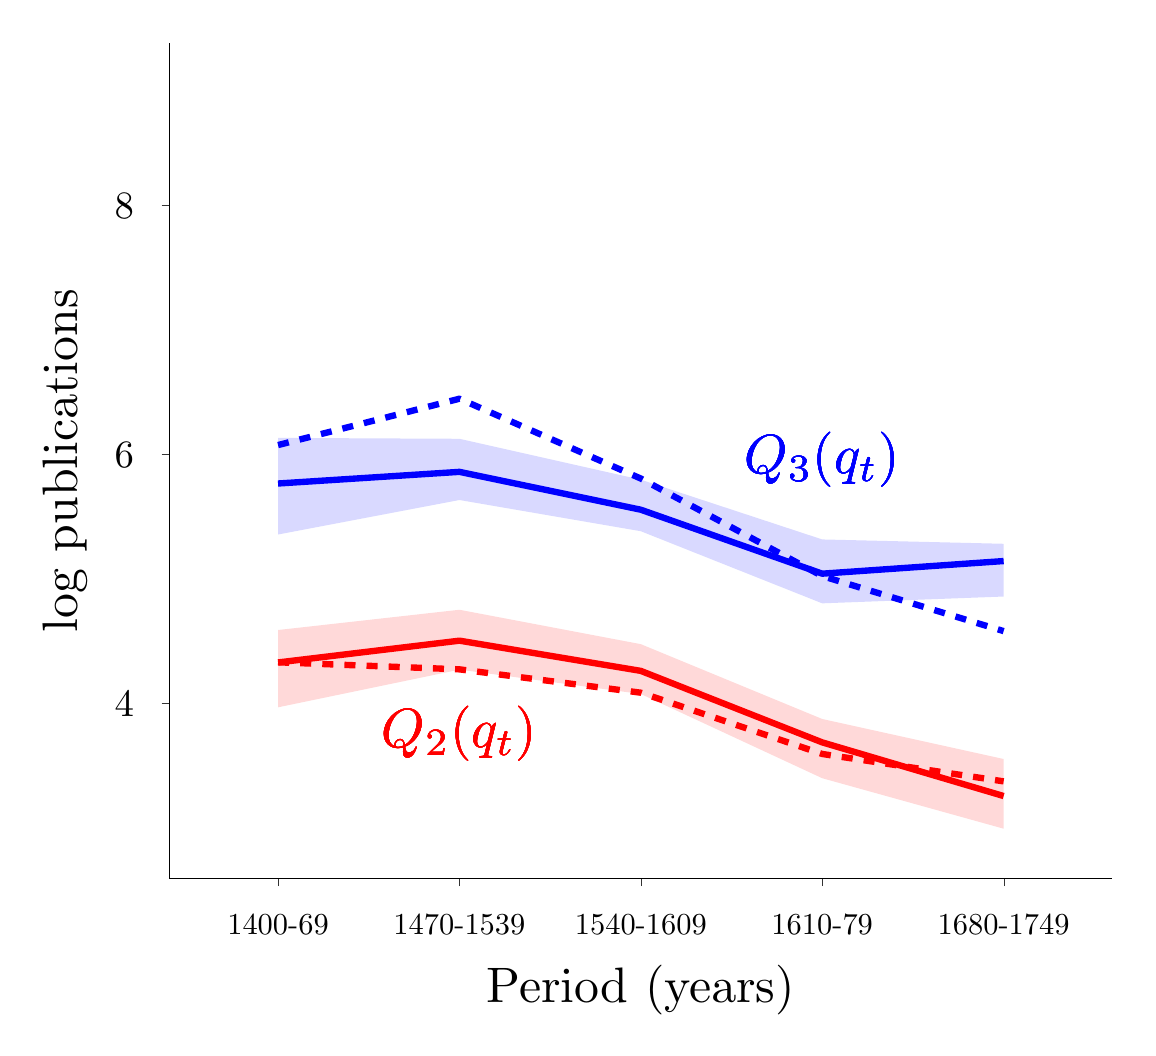
\begin{tikzpicture}[x=1pt,y=1pt]
\definecolor{fillColor}{RGB}{255,255,255}
\path[use as bounding box,fill=fillColor,fill opacity=0.00] (0,0) rectangle (397.48,361.35);
\begin{scope}
\path[clip] (  0.00,  0.00) rectangle (397.48,361.35);
\definecolor{drawColor}{RGB}{255,255,255}
\definecolor{fillColor}{RGB}{255,255,255}

\path[draw=drawColor,line width= 0.1pt,line join=round,line cap=round,fill=fillColor] (  0.00,  0.00) rectangle (397.48,361.35);
\end{scope}
\begin{scope}
\path[clip] ( 51.14, 53.86) rectangle (391.98,355.85);
\definecolor{fillColor}{RGB}{255,255,255}

\path[fill=fillColor] ( 51.14, 53.86) rectangle (391.98,355.85);
\definecolor{fillColor}{RGB}{255,0,0}

\path[fill=fillColor,fill opacity=0.15] ( 90.47,143.69) --
	(156.02,151.01) --
	(221.56,138.58) --
	(287.11,111.54) --
	(352.66, 97.08) --
	(352.66, 71.90) --
	(287.11, 90.14) --
	(221.56,120.58) --
	(156.02,129.37) --
	( 90.47,115.76) --
	cycle;

\path[] ( 90.47,143.69) --
	(156.02,151.01) --
	(221.56,138.58) --
	(287.11,111.54) --
	(352.66, 97.08);

\path[] (352.66, 71.90) --
	(287.11, 90.14) --
	(221.56,120.58) --
	(156.02,129.37) --
	( 90.47,115.76);
\definecolor{drawColor}{RGB}{255,0,0}

\path[draw=drawColor,line width= 2.3pt,line join=round] ( 90.47,131.97) --
	(156.02,139.84) --
	(221.56,128.92) --
	(287.11,103.09) --
	(352.66, 83.70);

\path[draw=drawColor,line width= 2.3pt,dash pattern=on 4pt off 4pt ,line join=round] ( 90.47,132.03) --
	(156.02,129.48) --
	(221.56,121.04) --
	(287.11, 98.90) --
	(352.66, 89.00);
\definecolor{fillColor}{RGB}{0,0,255}

\path[fill=fillColor,fill opacity=0.15] ( 90.47,213.11) --
	(156.02,212.79) --
	(221.56,198.01) --
	(287.11,176.42) --
	(352.66,174.85) --
	(352.66,155.79) --
	(287.11,153.33) --
	(221.56,179.39) --
	(156.02,190.67) --
	( 90.47,178.20) --
	cycle;

\path[] ( 90.47,213.11) --
	(156.02,212.79) --
	(221.56,198.01) --
	(287.11,176.42) --
	(352.66,174.85);

\path[] (352.66,155.79) --
	(287.11,153.33) --
	(221.56,179.39) --
	(156.02,190.67) --
	( 90.47,178.20);
\definecolor{drawColor}{RGB}{0,0,255}

\path[draw=drawColor,line width= 2.3pt,line join=round] ( 90.47,196.63) --
	(156.02,200.84) --
	(221.56,187.16) --
	(287.11,164.05) --
	(352.66,168.61);

\path[draw=drawColor,line width= 2.3pt,dash pattern=on 4pt off 4pt ,line join=round] ( 90.47,210.52) --
	(156.02,227.27) --
	(221.56,198.42) --
	(287.11,163.18) --
	(352.66,143.30);

\node[text=drawColor,anchor=base,inner sep=0pt, outer sep=0pt, scale=  1.99] at (287.11,200.25) {$Q_3(q_t)$};

\node[text=drawColor,anchor=base,inner sep=0pt, outer sep=0pt, scale=  1.99] at (287.11,200.25) {$Q_3(q_t)$};

\node[text=drawColor,anchor=base,inner sep=0pt, outer sep=0pt, scale=  1.99] at (287.11,200.25) {$Q_3(q_t)$};

\node[text=drawColor,anchor=base,inner sep=0pt, outer sep=0pt, scale=  1.99] at (287.11,200.25) {$Q_3(q_t)$};

\node[text=drawColor,anchor=base,inner sep=0pt, outer sep=0pt, scale=  1.99] at (287.11,200.25) {$Q_3(q_t)$};
\definecolor{drawColor}{RGB}{255,0,0}

\node[text=drawColor,anchor=base,inner sep=0pt, outer sep=0pt, scale=  1.99] at (156.02,101.23) {$Q_2(q_t)$};

\node[text=drawColor,anchor=base,inner sep=0pt, outer sep=0pt, scale=  1.99] at (156.02,101.23) {$Q_2(q_t)$};

\node[text=drawColor,anchor=base,inner sep=0pt, outer sep=0pt, scale=  1.99] at (156.02,101.23) {$Q_2(q_t)$};

\node[text=drawColor,anchor=base,inner sep=0pt, outer sep=0pt, scale=  1.99] at (156.02,101.23) {$Q_2(q_t)$};

\node[text=drawColor,anchor=base,inner sep=0pt, outer sep=0pt, scale=  1.99] at (156.02,101.23) {$Q_2(q_t)$};
\end{scope}
\begin{scope}
\path[clip] (  0.00,  0.00) rectangle (397.48,361.35);
\definecolor{drawColor}{RGB}{0,0,0}

\path[draw=drawColor,line width= 0.1pt,line join=round] ( 51.14, 53.86) --
	( 51.14,355.85);
\end{scope}
\begin{scope}
\path[clip] (  0.00,  0.00) rectangle (397.48,361.35);
\definecolor{drawColor}{RGB}{0,0,0}

\node[text=drawColor,anchor=base east,inner sep=0pt, outer sep=0pt, scale=  1.40] at ( 38.39,112.27) {4};

\node[text=drawColor,anchor=base east,inner sep=0pt, outer sep=0pt, scale=  1.40] at ( 38.39,202.28) {6};

\node[text=drawColor,anchor=base east,inner sep=0pt, outer sep=0pt, scale=  1.40] at ( 38.39,292.30) {8};
\end{scope}
\begin{scope}
\path[clip] (  0.00,  0.00) rectangle (397.48,361.35);
\definecolor{drawColor}{gray}{0.20}

\path[draw=drawColor,line width= 0.1pt,line join=round] ( 48.39,117.09) --
	( 51.14,117.09);

\path[draw=drawColor,line width= 0.1pt,line join=round] ( 48.39,207.11) --
	( 51.14,207.11);

\path[draw=drawColor,line width= 0.1pt,line join=round] ( 48.39,297.12) --
	( 51.14,297.12);
\end{scope}
\begin{scope}
\path[clip] (  0.00,  0.00) rectangle (397.48,361.35);
\definecolor{drawColor}{RGB}{0,0,0}

\path[draw=drawColor,line width= 0.1pt,line join=round] ( 51.14, 53.86) --
	(391.98, 53.86);
\end{scope}
\begin{scope}
\path[clip] (  0.00,  0.00) rectangle (397.48,361.35);
\definecolor{drawColor}{gray}{0.20}

\path[draw=drawColor,line width= 0.1pt,line join=round] ( 90.47, 51.11) --
	( 90.47, 53.86);

\path[draw=drawColor,line width= 0.1pt,line join=round] (156.02, 51.11) --
	(156.02, 53.86);

\path[draw=drawColor,line width= 0.1pt,line join=round] (221.56, 51.11) --
	(221.56, 53.86);

\path[draw=drawColor,line width= 0.1pt,line join=round] (287.11, 51.11) --
	(287.11, 53.86);

\path[draw=drawColor,line width= 0.1pt,line join=round] (352.66, 51.11) --
	(352.66, 53.86);
\end{scope}
\begin{scope}
\path[clip] (  0.00,  0.00) rectangle (397.48,361.35);
\definecolor{drawColor}{RGB}{0,0,0}

\node[text=drawColor,anchor=base,inner sep=0pt, outer sep=0pt, scale=  1.10] at ( 90.47, 33.53) {1400-69};

\node[text=drawColor,anchor=base,inner sep=0pt, outer sep=0pt, scale=  1.10] at (156.02, 33.53) {1470-1539};

\node[text=drawColor,anchor=base,inner sep=0pt, outer sep=0pt, scale=  1.10] at (221.56, 33.53) {1540-1609};

\node[text=drawColor,anchor=base,inner sep=0pt, outer sep=0pt, scale=  1.10] at (287.11, 33.53) {1610-79};

\node[text=drawColor,anchor=base,inner sep=0pt, outer sep=0pt, scale=  1.10] at (352.66, 33.53) {1680-1749};
\end{scope}
\begin{scope}
\path[clip] (  0.00,  0.00) rectangle (397.48,361.35);
\definecolor{drawColor}{RGB}{0,0,0}

\node[text=drawColor,anchor=base,inner sep=0pt, outer sep=0pt, scale=  1.80] at (221.56,  9.00) {Period (years)};
\end{scope}
\begin{scope}
\path[clip] (  0.00,  0.00) rectangle (397.48,361.35);
\definecolor{drawColor}{RGB}{0,0,0}

\node[text=drawColor,rotate= 90.00,anchor=base,inner sep=0pt, outer sep=0pt, scale=  1.80] at ( 17.90,204.86) {log publications};
\end{scope}
\end{tikzpicture}
}
}\hspace{-6mm}
\parbox{.49\textwidth}{
		\centering
{Share of censored scholars $\overline{\beta}m_t$\\
\textcolor{white}{a}}

\scalebox{0.55}{% Created by tikzDevice version 0.12.3.1 on 2022-09-19 22:27:54
% !TEX encoding = UTF-8 Unicode
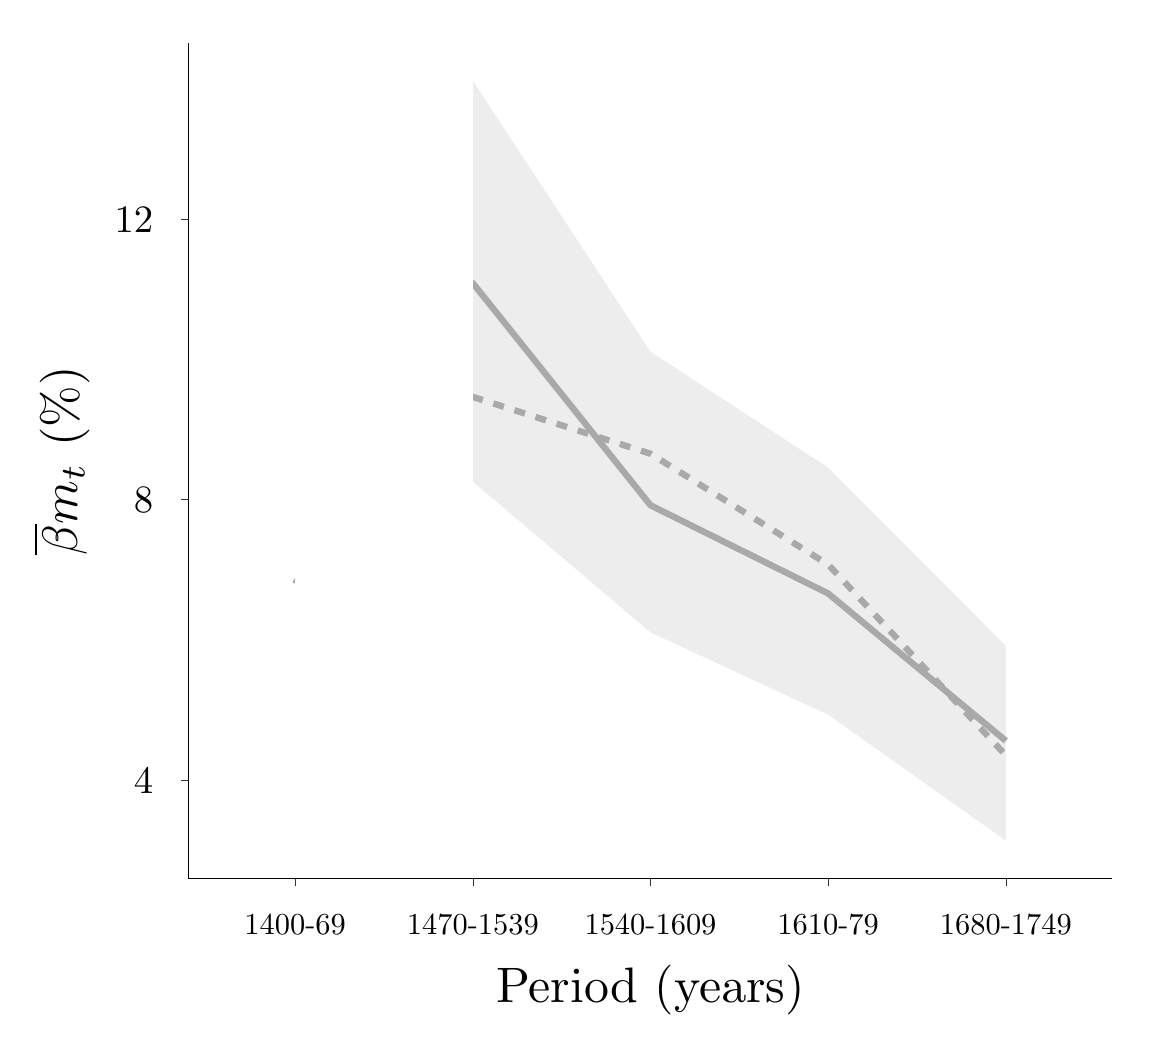
\begin{tikzpicture}[x=1pt,y=1pt]
\definecolor{fillColor}{RGB}{255,255,255}
\path[use as bounding box,fill=fillColor,fill opacity=0.00] (0,0) rectangle (397.48,361.35);
\begin{scope}
\path[clip] (  0.00,  0.00) rectangle (397.48,361.35);
\definecolor{drawColor}{RGB}{255,255,255}
\definecolor{fillColor}{RGB}{255,255,255}

\path[draw=drawColor,line width= 0.1pt,line join=round,line cap=round,fill=fillColor] (  0.00,  0.00) rectangle (397.48,361.35);
\end{scope}
\begin{scope}
\path[clip] ( 58.14, 53.86) rectangle (391.98,355.85);
\definecolor{fillColor}{RGB}{255,255,255}

\path[fill=fillColor] ( 58.14, 53.86) rectangle (391.98,355.85);
\definecolor{fillColor}{RGB}{169,169,169}

\path[fill=fillColor,fill opacity=0.20] ( 96.66,263.42) --
	(160.86,342.12) --
	(225.06,244.23) --
	(289.26,202.36) --
	(353.46,137.94) --
	(353.46, 67.59) --
	(289.26,113.10) --
	(225.06,142.83) --
	(160.86,197.32) --
	( 96.66, 75.91) --
	cycle;

\path[] ( 96.66,263.42) --
	(160.86,342.12) --
	(225.06,244.23) --
	(289.26,202.36) --
	(353.46,137.94);

\path[] (353.46, 67.59) --
	(289.26,113.10) --
	(225.06,142.83) --
	(160.86,197.32) --
	( 96.66, 75.91);
\definecolor{drawColor}{RGB}{169,169,169}

\path[draw=drawColor,line width= 2.3pt,line join=round] ( 96.66,160.39) --
	(160.86,269.05) --
	(225.06,188.77) --
	(289.26,156.89) --
	(353.46,103.64);

\path[draw=drawColor,line width= 2.3pt,dash pattern=on 4pt off 4pt ,line join=round] ( 96.66,226.06) --
	(160.86,227.93) --
	(225.06,207.39) --
	(289.26,167.35) --
	(353.46, 98.39);
\definecolor{fillColor}{RGB}{255,255,255}

\path[fill=fillColor] ( 96.66, 53.86) rectangle (160.86,355.85);

\path[fill=fillColor] ( 96.66, 53.86) rectangle (160.86,355.85);

\path[fill=fillColor] ( 96.66, 53.86) rectangle (160.86,355.85);

\path[fill=fillColor] ( 96.66, 53.86) rectangle (160.86,355.85);

\path[fill=fillColor] ( 96.66, 53.86) rectangle (160.86,355.85);
\end{scope}
\begin{scope}
\path[clip] (  0.00,  0.00) rectangle (397.48,361.35);
\definecolor{drawColor}{RGB}{0,0,0}

\path[draw=drawColor,line width= 0.1pt,line join=round] ( 58.14, 53.86) --
	( 58.14,355.85);
\end{scope}
\begin{scope}
\path[clip] (  0.00,  0.00) rectangle (397.48,361.35);
\definecolor{drawColor}{RGB}{0,0,0}

\node[text=drawColor,anchor=base east,inner sep=0pt, outer sep=0pt, scale=  1.40] at ( 45.39, 84.70) {4};

\node[text=drawColor,anchor=base east,inner sep=0pt, outer sep=0pt, scale=  1.40] at ( 45.39,186.09) {8};

\node[text=drawColor,anchor=base east,inner sep=0pt, outer sep=0pt, scale=  1.40] at ( 45.39,287.49) {12};
\end{scope}
\begin{scope}
\path[clip] (  0.00,  0.00) rectangle (397.48,361.35);
\definecolor{drawColor}{gray}{0.20}

\path[draw=drawColor,line width= 0.1pt,line join=round] ( 55.39, 89.52) --
	( 58.14, 89.52);

\path[draw=drawColor,line width= 0.1pt,line join=round] ( 55.39,190.91) --
	( 58.14,190.91);

\path[draw=drawColor,line width= 0.1pt,line join=round] ( 55.39,292.31) --
	( 58.14,292.31);
\end{scope}
\begin{scope}
\path[clip] (  0.00,  0.00) rectangle (397.48,361.35);
\definecolor{drawColor}{RGB}{0,0,0}

\path[draw=drawColor,line width= 0.1pt,line join=round] ( 58.14, 53.86) --
	(391.98, 53.86);
\end{scope}
\begin{scope}
\path[clip] (  0.00,  0.00) rectangle (397.48,361.35);
\definecolor{drawColor}{gray}{0.20}

\path[draw=drawColor,line width= 0.1pt,line join=round] ( 96.66, 51.11) --
	( 96.66, 53.86);

\path[draw=drawColor,line width= 0.1pt,line join=round] (160.86, 51.11) --
	(160.86, 53.86);

\path[draw=drawColor,line width= 0.1pt,line join=round] (225.06, 51.11) --
	(225.06, 53.86);

\path[draw=drawColor,line width= 0.1pt,line join=round] (289.26, 51.11) --
	(289.26, 53.86);

\path[draw=drawColor,line width= 0.1pt,line join=round] (353.46, 51.11) --
	(353.46, 53.86);
\end{scope}
\begin{scope}
\path[clip] (  0.00,  0.00) rectangle (397.48,361.35);
\definecolor{drawColor}{RGB}{0,0,0}

\node[text=drawColor,anchor=base,inner sep=0pt, outer sep=0pt, scale=  1.10] at ( 96.66, 33.53) {1400-69};

\node[text=drawColor,anchor=base,inner sep=0pt, outer sep=0pt, scale=  1.10] at (160.86, 33.53) {1470-1539};

\node[text=drawColor,anchor=base,inner sep=0pt, outer sep=0pt, scale=  1.10] at (225.06, 33.53) {1540-1609};

\node[text=drawColor,anchor=base,inner sep=0pt, outer sep=0pt, scale=  1.10] at (289.26, 33.53) {1610-79};

\node[text=drawColor,anchor=base,inner sep=0pt, outer sep=0pt, scale=  1.10] at (353.46, 33.53) {1680-1749};
\end{scope}
\begin{scope}
\path[clip] (  0.00,  0.00) rectangle (397.48,361.35);
\definecolor{drawColor}{RGB}{0,0,0}

\node[text=drawColor,anchor=base,inner sep=0pt, outer sep=0pt, scale=  1.80] at (225.06,  9.00) {Period (years)};
\end{scope}
\begin{scope}
\path[clip] (  0.00,  0.00) rectangle (397.48,361.35);
\definecolor{drawColor}{RGB}{0,0,0}

\node[text=drawColor,rotate= 90.00,anchor=base,inner sep=0pt, outer sep=0pt, scale=  1.80] at ( 17.90,204.86) {$\overline{\beta}m_t$ (\%)};
\end{scope}
\end{tikzpicture}
}
}

\vspace{10mm}
\hspace{0mm}
\parbox{.49\textwidth}{
		\centering
{Censored scholars quality:\\ \textcolor{red}{median $Q_2(q_t^R)$}, \textcolor{blue}{$75^{th}$ percentile $Q_3(q_t^R)$}}

\scalebox{0.55}{% Created by tikzDevice version 0.12.3.1 on 2022-09-19 22:27:53
% !TEX encoding = UTF-8 Unicode
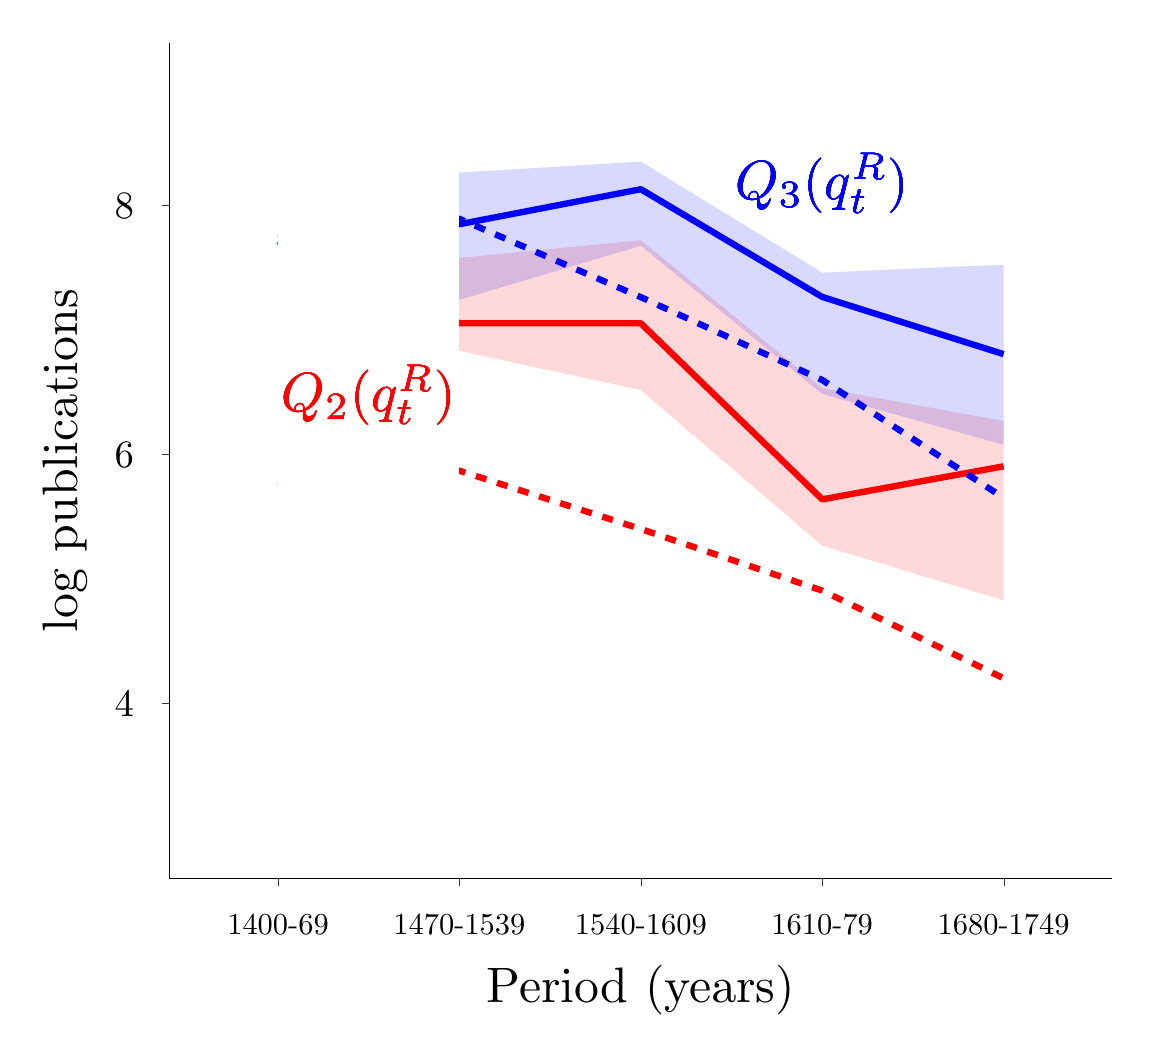
\begin{tikzpicture}[x=1pt,y=1pt]
\definecolor{fillColor}{RGB}{255,255,255}
\path[use as bounding box,fill=fillColor,fill opacity=0.00] (0,0) rectangle (397.48,361.35);
\begin{scope}
\path[clip] (  0.00,  0.00) rectangle (397.48,361.35);
\definecolor{drawColor}{RGB}{255,255,255}
\definecolor{fillColor}{RGB}{255,255,255}

\path[draw=drawColor,line width= 0.1pt,line join=round,line cap=round,fill=fillColor] (  0.00,  0.00) rectangle (397.48,361.35);
\end{scope}
\begin{scope}
\path[clip] ( 51.14, 53.86) rectangle (391.98,355.85);
\definecolor{fillColor}{RGB}{255,255,255}

\path[fill=fillColor] ( 51.14, 53.86) rectangle (391.98,355.85);
\definecolor{fillColor}{RGB}{255,0,0}

\path[fill=fillColor,fill opacity=0.15] ( 90.47,292.14) --
	(156.02,278.15) --
	(221.56,284.53) --
	(287.11,231.13) --
	(352.66,219.22) --
	(352.66,154.37) --
	(287.11,174.15) --
	(221.56,230.40) --
	(156.02,244.55) --
	( 90.47,254.76) --
	cycle;

\path[] ( 90.47,292.14) --
	(156.02,278.15) --
	(221.56,284.53) --
	(287.11,231.13) --
	(352.66,219.22);

\path[] (352.66,154.37) --
	(287.11,174.15) --
	(221.56,230.40) --
	(156.02,244.55) --
	( 90.47,254.76);
\definecolor{drawColor}{RGB}{255,0,0}

\path[draw=drawColor,line width= 2.3pt,line join=round] ( 90.47,284.23) --
	(156.02,254.56) --
	(221.56,254.52) --
	(287.11,190.91) --
	(352.66,202.85);

\path[draw=drawColor,line width= 2.3pt,dash pattern=on 4pt off 4pt ,line join=round] ( 90.47,195.87) --
	(156.02,201.25) --
	(221.56,180.20) --
	(287.11,157.93) --
	(352.66,126.27);
\definecolor{fillColor}{RGB}{0,0,255}

\path[fill=fillColor,fill opacity=0.15] ( 90.47,325.49) --
	(156.02,308.99) --
	(221.56,312.95) --
	(287.11,272.84) --
	(352.66,275.70) --
	(352.66,210.60) --
	(287.11,228.99) --
	(221.56,282.55) --
	(156.02,262.97) --
	( 90.47,278.47) --
	cycle;

\path[] ( 90.47,325.49) --
	(156.02,308.99) --
	(221.56,312.95) --
	(287.11,272.84) --
	(352.66,275.70);

\path[] (352.66,210.60) --
	(287.11,228.99) --
	(221.56,282.55) --
	(156.02,262.97) --
	( 90.47,278.47);
\definecolor{drawColor}{RGB}{0,0,255}

\path[draw=drawColor,line width= 2.3pt,line join=round] ( 90.47,291.49) --
	(156.02,290.33) --
	(221.56,302.97) --
	(287.11,264.05) --
	(352.66,243.37);

\path[draw=drawColor,line width= 2.3pt,dash pattern=on 4pt off 4pt ,line join=round] ( 90.47,285.04) --
	(156.02,292.27) --
	(221.56,263.97) --
	(287.11,234.03) --
	(352.66,191.46);
\definecolor{fillColor}{RGB}{255,255,255}

\path[fill=fillColor] ( 90.47, 53.86) rectangle (156.02,355.85);

\path[fill=fillColor] ( 90.47, 53.86) rectangle (156.02,355.85);

\path[fill=fillColor] ( 90.47, 53.86) rectangle (156.02,355.85);

\path[fill=fillColor] ( 90.47, 53.86) rectangle (156.02,355.85);

\path[fill=fillColor] ( 90.47, 53.86) rectangle (156.02,355.85);

\node[text=drawColor,anchor=base,inner sep=0pt, outer sep=0pt, scale=  1.99] at (287.11,299.26) {$Q_3(q_t^R)$};

\node[text=drawColor,anchor=base,inner sep=0pt, outer sep=0pt, scale=  1.99] at (287.11,299.26) {$Q_3(q_t^R)$};

\node[text=drawColor,anchor=base,inner sep=0pt, outer sep=0pt, scale=  1.99] at (287.11,299.26) {$Q_3(q_t^R)$};

\node[text=drawColor,anchor=base,inner sep=0pt, outer sep=0pt, scale=  1.99] at (287.11,299.26) {$Q_3(q_t^R)$};

\node[text=drawColor,anchor=base,inner sep=0pt, outer sep=0pt, scale=  1.99] at (287.11,299.26) {$Q_3(q_t^R)$};
\definecolor{drawColor}{RGB}{255,0,0}

\node[text=drawColor,anchor=base,inner sep=0pt, outer sep=0pt, scale=  1.99] at (123.25,222.75) {$Q_2(q_t^R)$};

\node[text=drawColor,anchor=base,inner sep=0pt, outer sep=0pt, scale=  1.99] at (123.25,222.75) {$Q_2(q_t^R)$};

\node[text=drawColor,anchor=base,inner sep=0pt, outer sep=0pt, scale=  1.99] at (123.25,222.75) {$Q_2(q_t^R)$};

\node[text=drawColor,anchor=base,inner sep=0pt, outer sep=0pt, scale=  1.99] at (123.25,222.75) {$Q_2(q_t^R)$};

\node[text=drawColor,anchor=base,inner sep=0pt, outer sep=0pt, scale=  1.99] at (123.25,222.75) {$Q_2(q_t^R)$};
\end{scope}
\begin{scope}
\path[clip] (  0.00,  0.00) rectangle (397.48,361.35);
\definecolor{drawColor}{RGB}{0,0,0}

\path[draw=drawColor,line width= 0.1pt,line join=round] ( 51.14, 53.86) --
	( 51.14,355.85);
\end{scope}
\begin{scope}
\path[clip] (  0.00,  0.00) rectangle (397.48,361.35);
\definecolor{drawColor}{RGB}{0,0,0}

\node[text=drawColor,anchor=base east,inner sep=0pt, outer sep=0pt, scale=  1.40] at ( 38.39,112.27) {4};

\node[text=drawColor,anchor=base east,inner sep=0pt, outer sep=0pt, scale=  1.40] at ( 38.39,202.28) {6};

\node[text=drawColor,anchor=base east,inner sep=0pt, outer sep=0pt, scale=  1.40] at ( 38.39,292.30) {8};
\end{scope}
\begin{scope}
\path[clip] (  0.00,  0.00) rectangle (397.48,361.35);
\definecolor{drawColor}{gray}{0.20}

\path[draw=drawColor,line width= 0.1pt,line join=round] ( 48.39,117.09) --
	( 51.14,117.09);

\path[draw=drawColor,line width= 0.1pt,line join=round] ( 48.39,207.11) --
	( 51.14,207.11);

\path[draw=drawColor,line width= 0.1pt,line join=round] ( 48.39,297.12) --
	( 51.14,297.12);
\end{scope}
\begin{scope}
\path[clip] (  0.00,  0.00) rectangle (397.48,361.35);
\definecolor{drawColor}{RGB}{0,0,0}

\path[draw=drawColor,line width= 0.1pt,line join=round] ( 51.14, 53.86) --
	(391.98, 53.86);
\end{scope}
\begin{scope}
\path[clip] (  0.00,  0.00) rectangle (397.48,361.35);
\definecolor{drawColor}{gray}{0.20}

\path[draw=drawColor,line width= 0.1pt,line join=round] ( 90.47, 51.11) --
	( 90.47, 53.86);

\path[draw=drawColor,line width= 0.1pt,line join=round] (156.02, 51.11) --
	(156.02, 53.86);

\path[draw=drawColor,line width= 0.1pt,line join=round] (221.56, 51.11) --
	(221.56, 53.86);

\path[draw=drawColor,line width= 0.1pt,line join=round] (287.11, 51.11) --
	(287.11, 53.86);

\path[draw=drawColor,line width= 0.1pt,line join=round] (352.66, 51.11) --
	(352.66, 53.86);
\end{scope}
\begin{scope}
\path[clip] (  0.00,  0.00) rectangle (397.48,361.35);
\definecolor{drawColor}{RGB}{0,0,0}

\node[text=drawColor,anchor=base,inner sep=0pt, outer sep=0pt, scale=  1.10] at ( 90.47, 33.53) {1400-69};

\node[text=drawColor,anchor=base,inner sep=0pt, outer sep=0pt, scale=  1.10] at (156.02, 33.53) {1470-1539};

\node[text=drawColor,anchor=base,inner sep=0pt, outer sep=0pt, scale=  1.10] at (221.56, 33.53) {1540-1609};

\node[text=drawColor,anchor=base,inner sep=0pt, outer sep=0pt, scale=  1.10] at (287.11, 33.53) {1610-79};

\node[text=drawColor,anchor=base,inner sep=0pt, outer sep=0pt, scale=  1.10] at (352.66, 33.53) {1680-1749};
\end{scope}
\begin{scope}
\path[clip] (  0.00,  0.00) rectangle (397.48,361.35);
\definecolor{drawColor}{RGB}{0,0,0}

\node[text=drawColor,anchor=base,inner sep=0pt, outer sep=0pt, scale=  1.80] at (221.56,  9.00) {Period (years)};
\end{scope}
\begin{scope}
\path[clip] (  0.00,  0.00) rectangle (397.48,361.35);
\definecolor{drawColor}{RGB}{0,0,0}

\node[text=drawColor,rotate= 90.00,anchor=base,inner sep=0pt, outer sep=0pt, scale=  1.80] at ( 17.90,204.86) {log publications};
\end{scope}
\end{tikzpicture}
 }
}\hspace{-4mm}
\parbox{.49\textwidth}{
		\centering
{Non-censored scholars
quality:\\ \textcolor{red}{median $Q_2(q_t^{NC})$}, \textcolor{blue}{$75^{th} $ percentile $Q_3(q_t^{NC})$}}

\scalebox{0.55}{% Created by tikzDevice version 0.12.3.1 on 2022-09-19 22:27:53
% !TEX encoding = UTF-8 Unicode
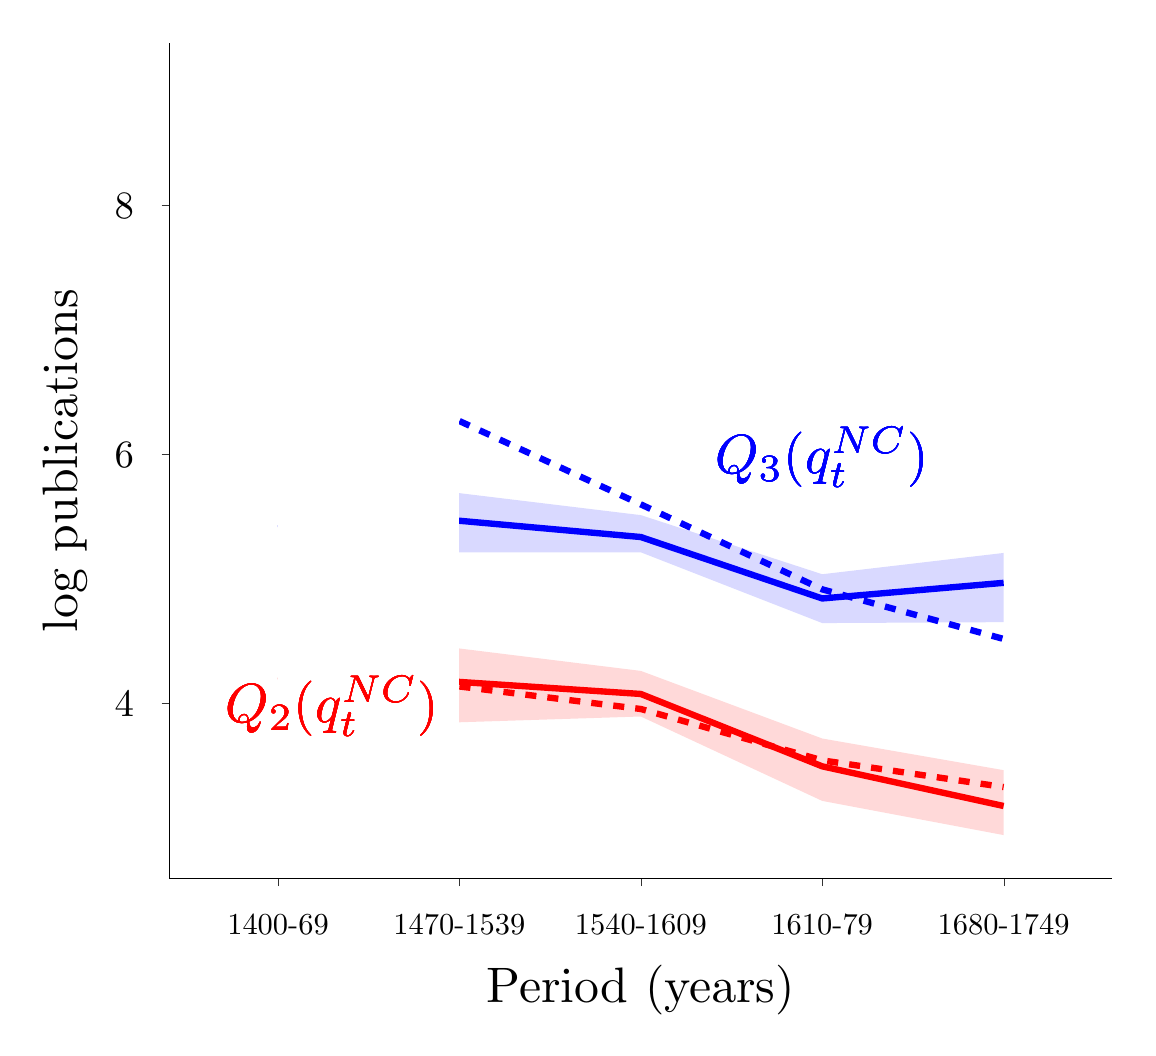
\begin{tikzpicture}[x=1pt,y=1pt]
\definecolor{fillColor}{RGB}{255,255,255}
\path[use as bounding box,fill=fillColor,fill opacity=0.00] (0,0) rectangle (397.48,361.35);
\begin{scope}
\path[clip] (  0.00,  0.00) rectangle (397.48,361.35);
\definecolor{drawColor}{RGB}{255,255,255}
\definecolor{fillColor}{RGB}{255,255,255}

\path[draw=drawColor,line width= 0.1pt,line join=round,line cap=round,fill=fillColor] (  0.00,  0.00) rectangle (397.48,361.35);
\end{scope}
\begin{scope}
\path[clip] ( 51.14, 53.86) rectangle (391.98,355.85);
\definecolor{fillColor}{RGB}{255,255,255}

\path[fill=fillColor] ( 51.14, 53.86) rectangle (391.98,355.85);
\definecolor{fillColor}{RGB}{255,0,0}

\path[fill=fillColor,fill opacity=0.15] ( 90.47,136.22) --
	(156.02,137.02) --
	(221.56,128.92) --
	(287.11,104.49) --
	(352.66, 93.05) --
	(352.66, 69.59) --
	(287.11, 81.94) --
	(221.56,112.44) --
	(156.02,110.35) --
	( 90.47,106.78) --
	cycle;

\path[] ( 90.47,136.22) --
	(156.02,137.02) --
	(221.56,128.92) --
	(287.11,104.49) --
	(352.66, 93.05);

\path[] (352.66, 69.59) --
	(287.11, 81.94) --
	(221.56,112.44) --
	(156.02,110.35) --
	( 90.47,106.78);
\definecolor{drawColor}{RGB}{255,0,0}

\path[draw=drawColor,line width= 2.3pt,line join=round] ( 90.47,126.97) --
	(156.02,124.94) --
	(221.56,120.58) --
	(287.11, 94.43) --
	(352.66, 80.10);

\path[draw=drawColor,line width= 2.3pt,dash pattern=on 4pt off 4pt ,line join=round] (156.02,123.30) --
	(221.56,115.15) --
	(287.11, 96.59) --
	(352.66, 86.95);
\definecolor{fillColor}{RGB}{0,0,255}

\path[fill=fillColor,fill opacity=0.15] ( 90.47,199.10) --
	(156.02,193.15) --
	(221.56,185.21) --
	(287.11,163.85) --
	(352.66,171.54) --
	(352.66,146.53) --
	(287.11,146.20) --
	(221.56,171.77) --
	(156.02,171.76) --
	( 90.47,164.34) --
	cycle;

\path[] ( 90.47,199.10) --
	(156.02,193.15) --
	(221.56,185.21) --
	(287.11,163.85) --
	(352.66,171.54);

\path[] (352.66,146.53) --
	(287.11,146.20) --
	(221.56,171.77) --
	(156.02,171.76) --
	( 90.47,164.34);
\definecolor{drawColor}{RGB}{0,0,255}

\path[draw=drawColor,line width= 2.3pt,line join=round] ( 90.47,180.48) --
	(156.02,183.17) --
	(221.56,177.29) --
	(287.11,155.09) --
	(352.66,160.74);

\path[draw=drawColor,line width= 2.3pt,dash pattern=on 4pt off 4pt ,line join=round] (156.02,219.20) --
	(221.56,189.09) --
	(287.11,158.39) --
	(352.66,140.46);
\definecolor{fillColor}{RGB}{255,255,255}

\path[fill=fillColor] ( 90.47, 53.86) rectangle (156.02,355.85);

\path[fill=fillColor] ( 90.47, 53.86) rectangle (156.02,355.85);

\path[fill=fillColor] ( 90.47, 53.86) rectangle (156.02,355.85);

\path[fill=fillColor] ( 90.47, 53.86) rectangle (156.02,355.85);

\path[fill=fillColor] ( 90.47, 53.86) rectangle (156.02,355.85);

\node[text=drawColor,anchor=base,inner sep=0pt, outer sep=0pt, scale=  1.99] at (287.11,200.25) {$Q_3(q_t^{NC})$};

\node[text=drawColor,anchor=base,inner sep=0pt, outer sep=0pt, scale=  1.99] at (287.11,200.25) {$Q_3(q_t^{NC})$};

\node[text=drawColor,anchor=base,inner sep=0pt, outer sep=0pt, scale=  1.99] at (287.11,200.25) {$Q_3(q_t^{NC})$};

\node[text=drawColor,anchor=base,inner sep=0pt, outer sep=0pt, scale=  1.99] at (287.11,200.25) {$Q_3(q_t^{NC})$};

\node[text=drawColor,anchor=base,inner sep=0pt, outer sep=0pt, scale=  1.99] at (287.11,200.25) {$Q_3(q_t^{NC})$};
\definecolor{drawColor}{RGB}{255,0,0}

\node[text=drawColor,anchor=base,inner sep=0pt, outer sep=0pt, scale=  1.99] at (110.14,110.23) {$Q_2(q_t^{NC})$};

\node[text=drawColor,anchor=base,inner sep=0pt, outer sep=0pt, scale=  1.99] at (110.14,110.23) {$Q_2(q_t^{NC})$};

\node[text=drawColor,anchor=base,inner sep=0pt, outer sep=0pt, scale=  1.99] at (110.14,110.23) {$Q_2(q_t^{NC})$};

\node[text=drawColor,anchor=base,inner sep=0pt, outer sep=0pt, scale=  1.99] at (110.14,110.23) {$Q_2(q_t^{NC})$};

\node[text=drawColor,anchor=base,inner sep=0pt, outer sep=0pt, scale=  1.99] at (110.14,110.23) {$Q_2(q_t^{NC})$};
\end{scope}
\begin{scope}
\path[clip] (  0.00,  0.00) rectangle (397.48,361.35);
\definecolor{drawColor}{RGB}{0,0,0}

\path[draw=drawColor,line width= 0.1pt,line join=round] ( 51.14, 53.86) --
	( 51.14,355.85);
\end{scope}
\begin{scope}
\path[clip] (  0.00,  0.00) rectangle (397.48,361.35);
\definecolor{drawColor}{RGB}{0,0,0}

\node[text=drawColor,anchor=base east,inner sep=0pt, outer sep=0pt, scale=  1.40] at ( 38.39,112.27) {4};

\node[text=drawColor,anchor=base east,inner sep=0pt, outer sep=0pt, scale=  1.40] at ( 38.39,202.28) {6};

\node[text=drawColor,anchor=base east,inner sep=0pt, outer sep=0pt, scale=  1.40] at ( 38.39,292.30) {8};
\end{scope}
\begin{scope}
\path[clip] (  0.00,  0.00) rectangle (397.48,361.35);
\definecolor{drawColor}{gray}{0.20}

\path[draw=drawColor,line width= 0.1pt,line join=round] ( 48.39,117.09) --
	( 51.14,117.09);

\path[draw=drawColor,line width= 0.1pt,line join=round] ( 48.39,207.11) --
	( 51.14,207.11);

\path[draw=drawColor,line width= 0.1pt,line join=round] ( 48.39,297.12) --
	( 51.14,297.12);
\end{scope}
\begin{scope}
\path[clip] (  0.00,  0.00) rectangle (397.48,361.35);
\definecolor{drawColor}{RGB}{0,0,0}

\path[draw=drawColor,line width= 0.1pt,line join=round] ( 51.14, 53.86) --
	(391.98, 53.86);
\end{scope}
\begin{scope}
\path[clip] (  0.00,  0.00) rectangle (397.48,361.35);
\definecolor{drawColor}{gray}{0.20}

\path[draw=drawColor,line width= 0.1pt,line join=round] ( 90.47, 51.11) --
	( 90.47, 53.86);

\path[draw=drawColor,line width= 0.1pt,line join=round] (156.02, 51.11) --
	(156.02, 53.86);

\path[draw=drawColor,line width= 0.1pt,line join=round] (221.56, 51.11) --
	(221.56, 53.86);

\path[draw=drawColor,line width= 0.1pt,line join=round] (287.11, 51.11) --
	(287.11, 53.86);

\path[draw=drawColor,line width= 0.1pt,line join=round] (352.66, 51.11) --
	(352.66, 53.86);
\end{scope}
\begin{scope}
\path[clip] (  0.00,  0.00) rectangle (397.48,361.35);
\definecolor{drawColor}{RGB}{0,0,0}

\node[text=drawColor,anchor=base,inner sep=0pt, outer sep=0pt, scale=  1.10] at ( 90.47, 33.53) {1400-69};

\node[text=drawColor,anchor=base,inner sep=0pt, outer sep=0pt, scale=  1.10] at (156.02, 33.53) {1470-1539};

\node[text=drawColor,anchor=base,inner sep=0pt, outer sep=0pt, scale=  1.10] at (221.56, 33.53) {1540-1609};

\node[text=drawColor,anchor=base,inner sep=0pt, outer sep=0pt, scale=  1.10] at (287.11, 33.53) {1610-79};

\node[text=drawColor,anchor=base,inner sep=0pt, outer sep=0pt, scale=  1.10] at (352.66, 33.53) {1680-1749};
\end{scope}
\begin{scope}
\path[clip] (  0.00,  0.00) rectangle (397.48,361.35);
\definecolor{drawColor}{RGB}{0,0,0}

\node[text=drawColor,anchor=base,inner sep=0pt, outer sep=0pt, scale=  1.80] at (221.56,  9.00) {Period (years)};
\end{scope}
\begin{scope}
\path[clip] (  0.00,  0.00) rectangle (397.48,361.35);
\definecolor{drawColor}{RGB}{0,0,0}

\node[text=drawColor,rotate= 90.00,anchor=base,inner sep=0pt, outer sep=0pt, scale=  1.80] at ( 17.90,204.86) {log publications};
\end{scope}
\end{tikzpicture}
}
}
	\caption{Model fit (upper panels), over-identification checks (lower panels).\\ Data (solid) and simulations (dashed).}
	\label{fig:fit}
\end{figure}

%Note that our parameter estimates would be biased if the convergence forces, which imply larger growth rates for lower levels of knowledge, were not correctly taken into account by the model. In Appendix~\ref{O-app:robust-convergence} we show that the model matches well the publication dynamics of Great Britain, which lagged behind Italy in the fifteenth century.
%\section{The Decline of Italy and Convergence} \label{app:robust-convergence}
%In this paper we use a structural model to assess quantitatively the role of censorship in the decline in total publications per scholar in Italy. The credibility of our quantification depends on whether the convergence forces, which imply larger growth rates for lower levels of knowledge, are correctly taken into account by the model. If this was not the case, our parameter estimates would be biased.
%For example, if the model convergence forces were stronger than the actual ones, the estimated effect of censorship would be too large because of the need to keep the level of publications in Italy low

The model fit is reported in Figure~\ref{fig:fit}, upper panels. The simulated variables rarely lie outside the $95\%$ confidence interval of the data moments. %An exception is the $75^{th}$ percentile of the overall knowledge quality. This reflects that the underlying empirical distribution does not follow exactly a Fr\'echet distribution like in the model.

%As a test of the theory, we compare our results to empirical observations that were not used to identify the parameters. Looking at the quality of censored $q_t^R$ and non-censored authors $q_t^{NC}$ (Figure~\ref{fig:fit}, lower panels) is particularly interesting as it allows us to test whether printers choose their sector according to its (relative) quality.\footnote{The distribution of quality of censored and revolutionary authors is the same because censorship is random. The distribution of quality of non-censored authors  $q_t^{NC}$ is obtained by drawing from the distribution of $q^R_t$ with probability $p^{nc}$ and from the distribution of $q^C_t$ with probability $1-p^{nc}$, where $p^{nc}$ is the share of \textit{printed} books that are revolutionary.}  This mechanism is summarized by Equation (\ref{eq:sharer2}): the share of revolutionary authors can assume one and only one variable given the ratio of the quality in the two sectors. This ratio can be proxied by the ratio of censored to non-censored authors' quality, which we can measure in the data. Since the model fit well the dynamics of censored and non-censored authors, we can assert that Equation~(\ref{eq:sharer2}) is likely to hold in the data too. The model also predicts that the share of revolutionary ideas was increasing before $t=3$. This is consistent with the fact that the share of censored books was larger in the period 1470-1539 than 1400-1469. Moreover, the average difference in quality between censored and non-censored authors decreases from 3.60 in 1470-1539 to 1.46 in 1680-1749.

As a test of the theory, we compare our results to empirical observations that were not used to identify the parameters. Looking at the quality of censored $q_t^R$ and non-censored authors $q_t^{NC}$ (Figure~\ref{fig:fit}, lower panels) is particularly interesting.\footnote{The distribution of quality of censored and revolutionary authors is the same because censorship is random. The distribution of quality of non-censored authors  $q_t^{NC}$ is obtained by drawing from the distribution of $q^R_t$ with probability $p^{nc}$ and from the distribution of $q^C_t$ with probability $1-p^{nc}$, where $p^{nc}$ is the share of \textit{printed} books that are revolutionary.} This is because from the model's theoretical restrictions it follows that the observed share of censored authors and overall quality imply specific distributions of $q_t^R$ and $q_t^{NC}$ for a given parametrization.\footnote{Equation (\ref{eq:sharer2}) implies that the share of revolutionary authors can assume one and only one value given the ratio of quality in the two sectors $k^R_t$ and $k^C_t$. Since authors’ quality  in sector $j$ is strictly increasing in $k^j_t$, a given level of overall quality and share of censored authors can only be generated by two specific values of $k^R_t$ and $k^C_t$ for a specific parametrization. Finally, note that $k^R_t$ and $k^C_t$ are the model state variables: their value implies a specific quality of censored and non-censored authors.} Without targeting these moments in particular, the model matches them well, which gives credence to the model's mechanisms. The model also predicts that the share of revolutionary ideas was increasing before $t=3$. This is consistent with the fact that the share of censored books was larger in the period 1470-1539 than 1400-1469. Moreover, the average difference in quality between censored and non-censored authors decreases from 2.91 in 1470-1539 to 1.72 in 1680-1749.

As a second out of sample test of our theory, we compare the dynamics of publications in Great Britain with model simulations. Data for Great Britain are in Appendix~\ref{O-app:british}. We simulate the dynamics of publications by decreasing the initial conditions in the state of knowledge ($k^R_1,k^C_1$) used for Italy by $45\%$ to match the median number of log publications in Great Britain in $t=2$.\footnote{We consider $t=2$ and not $t=1$ because we have less than 20 published scholars for $t=1$.} The remaining parameters are set equal to those used for Italy, except for $\overline{\beta}$, which is set to 0 (no censorship). We also recompute the process for $\mu_t$ using GDP per capita. The results are shown in Figure~\ref{fig:Sq_uk}.


%UPDATED 29 AUG 2022=========================================================================================================================
\begin{figure}[htb]	
	\centering
	\hspace*{-1cm}
	
	% include second image
	\scalebox{0.36}{\input{sq_uk.tex} }
	
	\caption{Median scholars quality $Q_2(q_t)$. Blue: Great Britain. Red: Italy.  \\ Data (solid) and simulations (dashed). }
	\label{fig:Sq_uk}
\end{figure}

Simulations of median log publications in Great Britain are relatively close to their data counterpart, despite we did not used them in the estimation procedure. The model shows the ability to match well the British data when the initial conditions are set to a level lower than the Italian case. This result supports the claim that the model predicts correctly the catching up and overtaking of Great Britain, through a mix of convergence forces acting in the dynamics of $m_t$, differences in the  exogenous process of $\mu_t$, and the presence of censorship in Italy.


\subsubsection*{The Role of Censorship in Knowledge Formation}

What is the role of the Catholic Church in the demise in knowledge production in early modern Italy? How much of this effect is driven by selection into the revolutionary/compliant sectors? In this section we answer these questions by comparing model simulations with and without censorship. This is done by setting the rate of censorship $\overline{\beta}$ to $0$ in the no-censorship scenario. Figure~\ref{fig:exp} illustrates the outcomes of the experiments.

%%%%%%%%%%%%%%%%%%%%%%%%%%%%%%%%%%%%%%
%Const. exp.  1
%%%%%%%%%%%%%%%%%%%%%%%%%%%%%%%%%%%%%%
%UPDATED 29 AUG 2022=========================================================================================================================
\begin{figure}[htb]	
	\centering
	\hspace*{-1cm}
	\begin{subfigure}{.49\textwidth}
		\centering
		% include first image
		\caption{Share of revolutionary scholars ($m_t$)\\\textcolor{white}{a}}
		\label{sf:ra}
		\scalebox{0.55}{% Created by tikzDevice version 0.12.3.1 on 2022-09-19 22:27:55
% !TEX encoding = UTF-8 Unicode
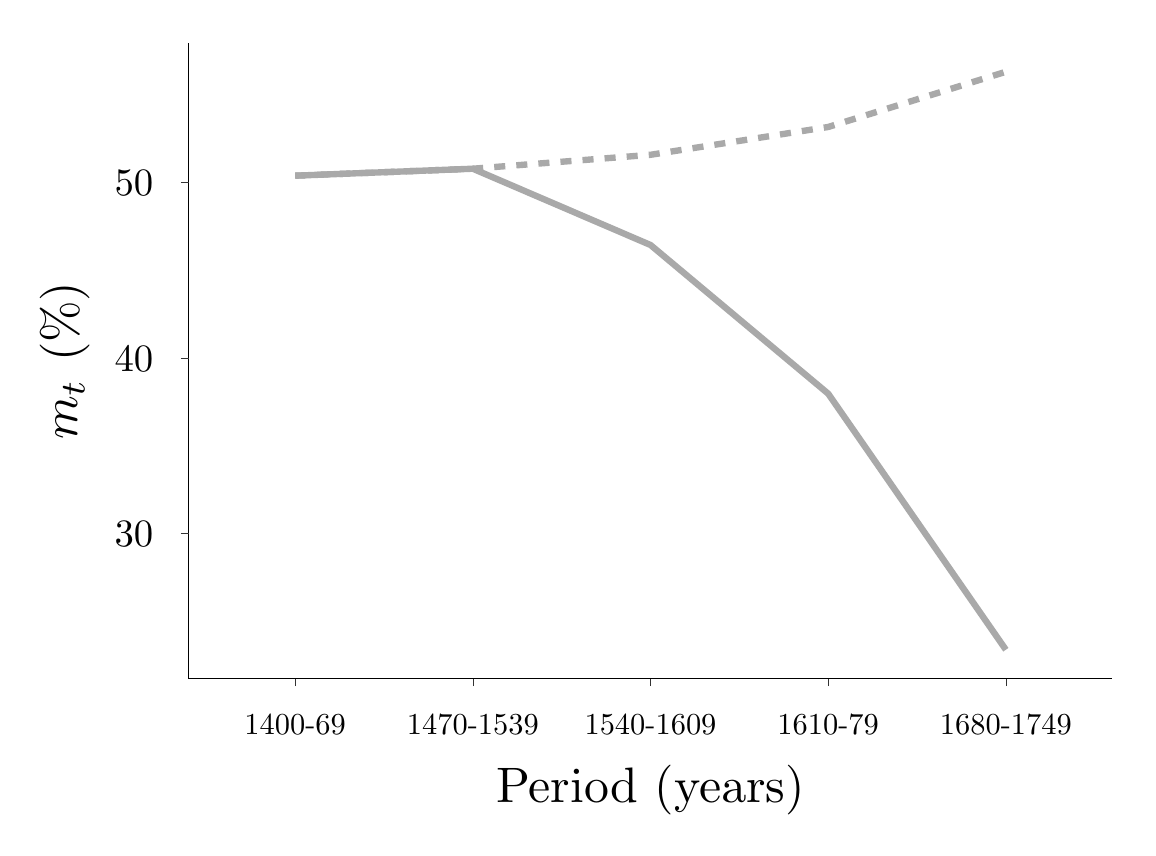
\begin{tikzpicture}[x=1pt,y=1pt]
\definecolor{fillColor}{RGB}{255,255,255}
\path[use as bounding box,fill=fillColor,fill opacity=0.00] (0,0) rectangle (397.48,289.08);
\begin{scope}
\path[clip] (  0.00,  0.00) rectangle (397.48,289.08);
\definecolor{drawColor}{RGB}{255,255,255}
\definecolor{fillColor}{RGB}{255,255,255}

\path[draw=drawColor,line width= 0.1pt,line join=round,line cap=round,fill=fillColor] (  0.00,  0.00) rectangle (397.48,289.08);
\end{scope}
\begin{scope}
\path[clip] ( 58.14, 53.86) rectangle (391.98,283.58);
\definecolor{fillColor}{RGB}{255,255,255}

\path[fill=fillColor] ( 58.14, 53.86) rectangle (391.98,283.58);
\definecolor{drawColor}{RGB}{169,169,169}

\path[draw=drawColor,line width= 2.3pt,line join=round] ( 96.66,235.59) --
	(160.86,238.11) --
	(225.06,210.55) --
	(289.26,156.83) --
	(353.46, 64.30);

\path[draw=drawColor,line width= 2.3pt,dash pattern=on 4pt off 4pt ,line join=round] ( 96.66,235.59) --
	(160.86,238.11) --
	(225.06,243.14) --
	(289.26,253.19) --
	(353.46,273.14);
\end{scope}
\begin{scope}
\path[clip] (  0.00,  0.00) rectangle (397.48,289.08);
\definecolor{drawColor}{RGB}{0,0,0}

\path[draw=drawColor,line width= 0.1pt,line join=round] ( 58.14, 53.86) --
	( 58.14,283.58);
\end{scope}
\begin{scope}
\path[clip] (  0.00,  0.00) rectangle (397.48,289.08);
\definecolor{drawColor}{RGB}{0,0,0}

\node[text=drawColor,anchor=base east,inner sep=0pt, outer sep=0pt, scale=  1.40] at ( 45.39,101.57) {30};

\node[text=drawColor,anchor=base east,inner sep=0pt, outer sep=0pt, scale=  1.40] at ( 45.39,164.91) {40};

\node[text=drawColor,anchor=base east,inner sep=0pt, outer sep=0pt, scale=  1.40] at ( 45.39,228.26) {50};
\end{scope}
\begin{scope}
\path[clip] (  0.00,  0.00) rectangle (397.48,289.08);
\definecolor{drawColor}{gray}{0.20}

\path[draw=drawColor,line width= 0.1pt,line join=round] ( 55.39,106.39) --
	( 58.14,106.39);

\path[draw=drawColor,line width= 0.1pt,line join=round] ( 55.39,169.73) --
	( 58.14,169.73);

\path[draw=drawColor,line width= 0.1pt,line join=round] ( 55.39,233.08) --
	( 58.14,233.08);
\end{scope}
\begin{scope}
\path[clip] (  0.00,  0.00) rectangle (397.48,289.08);
\definecolor{drawColor}{RGB}{0,0,0}

\path[draw=drawColor,line width= 0.1pt,line join=round] ( 58.14, 53.86) --
	(391.98, 53.86);
\end{scope}
\begin{scope}
\path[clip] (  0.00,  0.00) rectangle (397.48,289.08);
\definecolor{drawColor}{gray}{0.20}

\path[draw=drawColor,line width= 0.1pt,line join=round] ( 96.66, 51.11) --
	( 96.66, 53.86);

\path[draw=drawColor,line width= 0.1pt,line join=round] (160.86, 51.11) --
	(160.86, 53.86);

\path[draw=drawColor,line width= 0.1pt,line join=round] (225.06, 51.11) --
	(225.06, 53.86);

\path[draw=drawColor,line width= 0.1pt,line join=round] (289.26, 51.11) --
	(289.26, 53.86);

\path[draw=drawColor,line width= 0.1pt,line join=round] (353.46, 51.11) --
	(353.46, 53.86);
\end{scope}
\begin{scope}
\path[clip] (  0.00,  0.00) rectangle (397.48,289.08);
\definecolor{drawColor}{RGB}{0,0,0}

\node[text=drawColor,anchor=base,inner sep=0pt, outer sep=0pt, scale=  1.10] at ( 96.66, 33.53) {1400-69};

\node[text=drawColor,anchor=base,inner sep=0pt, outer sep=0pt, scale=  1.10] at (160.86, 33.53) {1470-1539};

\node[text=drawColor,anchor=base,inner sep=0pt, outer sep=0pt, scale=  1.10] at (225.06, 33.53) {1540-1609};

\node[text=drawColor,anchor=base,inner sep=0pt, outer sep=0pt, scale=  1.10] at (289.26, 33.53) {1610-79};

\node[text=drawColor,anchor=base,inner sep=0pt, outer sep=0pt, scale=  1.10] at (353.46, 33.53) {1680-1749};
\end{scope}
\begin{scope}
\path[clip] (  0.00,  0.00) rectangle (397.48,289.08);
\definecolor{drawColor}{RGB}{0,0,0}

\node[text=drawColor,anchor=base,inner sep=0pt, outer sep=0pt, scale=  1.80] at (225.06,  9.00) {Period (years)};
\end{scope}
\begin{scope}
\path[clip] (  0.00,  0.00) rectangle (397.48,289.08);
\definecolor{drawColor}{RGB}{0,0,0}

\node[text=drawColor,rotate= 90.00,anchor=base,inner sep=0pt, outer sep=0pt, scale=  1.80] at ( 17.90,168.72) {$m_t$ (\%)};
\end{scope}
\end{tikzpicture}
 }
	\end{subfigure}\hspace{-5mm}
	\begin{subfigure}{.49\textwidth}
		\centering
		% include second image
		\caption{\textcolor{blue}{Overall}, \textcolor{red}{revolutionary}\\ \textcolor{orange}{compliant} scholars quality}
		\label{sf:dq}
		\scalebox{0.55}{% Created by tikzDevice version 0.12.3.1 on 2022-09-19 22:27:55
% !TEX encoding = UTF-8 Unicode
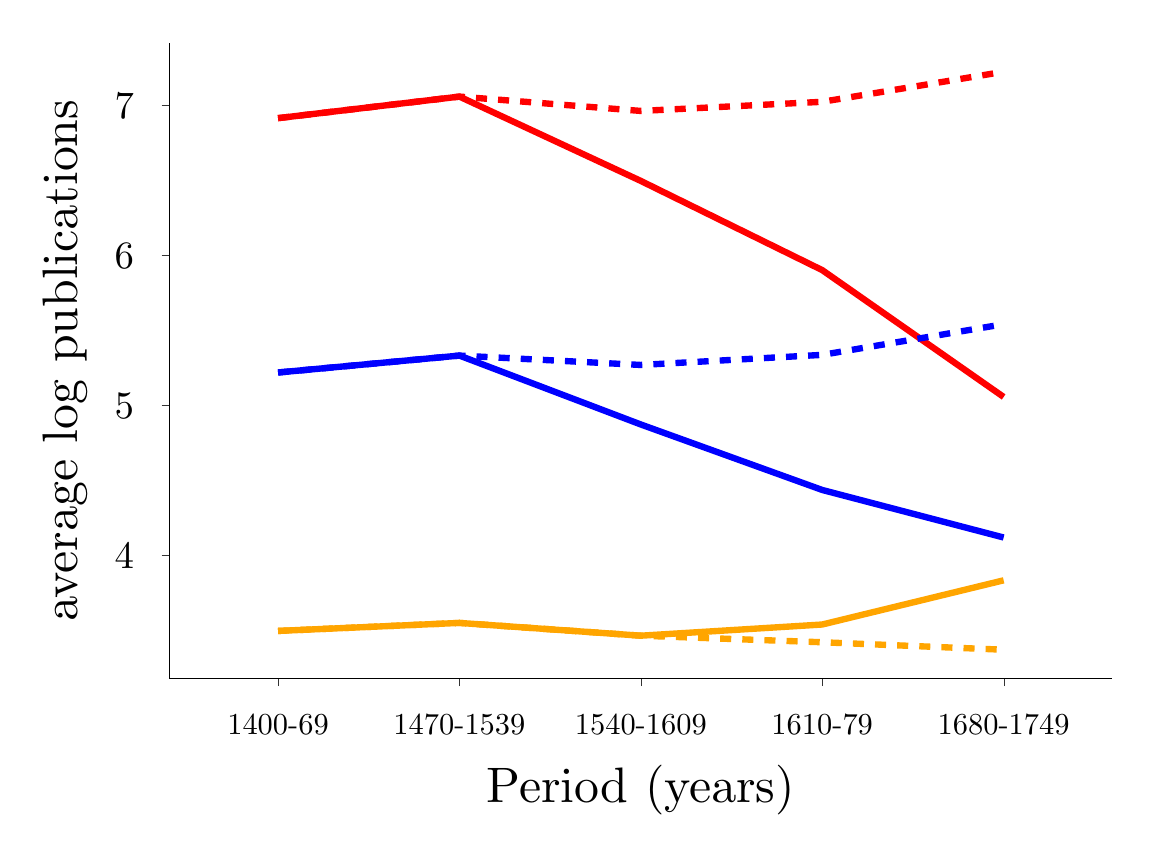
\begin{tikzpicture}[x=1pt,y=1pt]
\definecolor{fillColor}{RGB}{255,255,255}
\path[use as bounding box,fill=fillColor,fill opacity=0.00] (0,0) rectangle (397.48,289.08);
\begin{scope}
\path[clip] (  0.00,  0.00) rectangle (397.48,289.08);
\definecolor{drawColor}{RGB}{255,255,255}
\definecolor{fillColor}{RGB}{255,255,255}

\path[draw=drawColor,line width= 0.1pt,line join=round,line cap=round,fill=fillColor] (  0.00,  0.00) rectangle (397.48,289.08);
\end{scope}
\begin{scope}
\path[clip] ( 51.14, 53.86) rectangle (391.98,283.58);
\definecolor{fillColor}{RGB}{255,255,255}

\path[fill=fillColor] ( 51.14, 53.86) rectangle (391.98,283.58);
\definecolor{drawColor}{RGB}{255,0,0}

\path[draw=drawColor,line width= 2.3pt,line join=round] ( 90.47,256.38) --
	(156.02,264.17) --
	(221.56,233.70) --
	(287.11,201.47) --
	(352.66,155.64);

\path[draw=drawColor,line width= 2.3pt,dash pattern=on 4pt off 4pt ,line join=round] ( 90.47,256.38) --
	(156.02,264.17) --
	(221.56,258.99) --
	(287.11,262.29) --
	(352.66,273.14);
\definecolor{drawColor}{RGB}{0,0,255}

\path[draw=drawColor,line width= 2.3pt,line join=round] ( 90.47,164.47) --
	(156.02,170.59) --
	(221.56,145.69) --
	(287.11,122.03) --
	(352.66,104.85);

\path[draw=drawColor,line width= 2.3pt,dash pattern=on 4pt off 4pt ,line join=round] ( 90.47,164.47) --
	(156.02,170.59) --
	(221.56,167.20) --
	(287.11,170.85) --
	(352.66,181.93);
\definecolor{drawColor}{RGB}{255,165,0}

\path[draw=drawColor,line width= 2.3pt,line join=round] ( 90.47, 71.09) --
	(156.02, 73.99) --
	(221.56, 69.37) --
	(287.11, 73.41) --
	(352.66, 89.38);

\path[draw=drawColor,line width= 2.3pt,dash pattern=on 4pt off 4pt ,line join=round] ( 90.47, 71.09) --
	(156.02, 73.99) --
	(221.56, 69.37) --
	(287.11, 67.00) --
	(352.66, 64.30);
\end{scope}
\begin{scope}
\path[clip] (  0.00,  0.00) rectangle (397.48,289.08);
\definecolor{drawColor}{RGB}{0,0,0}

\path[draw=drawColor,line width= 0.1pt,line join=round] ( 51.14, 53.86) --
	( 51.14,283.58);
\end{scope}
\begin{scope}
\path[clip] (  0.00,  0.00) rectangle (397.48,289.08);
\definecolor{drawColor}{RGB}{0,0,0}

\node[text=drawColor,anchor=base east,inner sep=0pt, outer sep=0pt, scale=  1.40] at ( 38.39, 93.70) {4};

\node[text=drawColor,anchor=base east,inner sep=0pt, outer sep=0pt, scale=  1.40] at ( 38.39,147.89) {5};

\node[text=drawColor,anchor=base east,inner sep=0pt, outer sep=0pt, scale=  1.40] at ( 38.39,202.08) {6};

\node[text=drawColor,anchor=base east,inner sep=0pt, outer sep=0pt, scale=  1.40] at ( 38.39,256.27) {7};
\end{scope}
\begin{scope}
\path[clip] (  0.00,  0.00) rectangle (397.48,289.08);
\definecolor{drawColor}{gray}{0.20}

\path[draw=drawColor,line width= 0.1pt,line join=round] ( 48.39, 98.52) --
	( 51.14, 98.52);

\path[draw=drawColor,line width= 0.1pt,line join=round] ( 48.39,152.71) --
	( 51.14,152.71);

\path[draw=drawColor,line width= 0.1pt,line join=round] ( 48.39,206.90) --
	( 51.14,206.90);

\path[draw=drawColor,line width= 0.1pt,line join=round] ( 48.39,261.09) --
	( 51.14,261.09);
\end{scope}
\begin{scope}
\path[clip] (  0.00,  0.00) rectangle (397.48,289.08);
\definecolor{drawColor}{RGB}{0,0,0}

\path[draw=drawColor,line width= 0.1pt,line join=round] ( 51.14, 53.86) --
	(391.98, 53.86);
\end{scope}
\begin{scope}
\path[clip] (  0.00,  0.00) rectangle (397.48,289.08);
\definecolor{drawColor}{gray}{0.20}

\path[draw=drawColor,line width= 0.1pt,line join=round] ( 90.47, 51.11) --
	( 90.47, 53.86);

\path[draw=drawColor,line width= 0.1pt,line join=round] (156.02, 51.11) --
	(156.02, 53.86);

\path[draw=drawColor,line width= 0.1pt,line join=round] (221.56, 51.11) --
	(221.56, 53.86);

\path[draw=drawColor,line width= 0.1pt,line join=round] (287.11, 51.11) --
	(287.11, 53.86);

\path[draw=drawColor,line width= 0.1pt,line join=round] (352.66, 51.11) --
	(352.66, 53.86);
\end{scope}
\begin{scope}
\path[clip] (  0.00,  0.00) rectangle (397.48,289.08);
\definecolor{drawColor}{RGB}{0,0,0}

\node[text=drawColor,anchor=base,inner sep=0pt, outer sep=0pt, scale=  1.10] at ( 90.47, 33.53) {1400-69};

\node[text=drawColor,anchor=base,inner sep=0pt, outer sep=0pt, scale=  1.10] at (156.02, 33.53) {1470-1539};

\node[text=drawColor,anchor=base,inner sep=0pt, outer sep=0pt, scale=  1.10] at (221.56, 33.53) {1540-1609};

\node[text=drawColor,anchor=base,inner sep=0pt, outer sep=0pt, scale=  1.10] at (287.11, 33.53) {1610-79};

\node[text=drawColor,anchor=base,inner sep=0pt, outer sep=0pt, scale=  1.10] at (352.66, 33.53) {1680-1749};
\end{scope}
\begin{scope}
\path[clip] (  0.00,  0.00) rectangle (397.48,289.08);
\definecolor{drawColor}{RGB}{0,0,0}

\node[text=drawColor,anchor=base,inner sep=0pt, outer sep=0pt, scale=  1.80] at (221.56,  9.00) {Period (years)};
\end{scope}
\begin{scope}
\path[clip] (  0.00,  0.00) rectangle (397.48,289.08);
\definecolor{drawColor}{RGB}{0,0,0}

\node[text=drawColor,rotate= 90.00,anchor=base,inner sep=0pt, outer sep=0pt, scale=  1.80] at ( 17.90,168.72) {average log publications};
\end{scope}
\end{tikzpicture}
 }
	\end{subfigure}

	\caption{Baseline simulations (solid), simulations without censorship (dashed)}
	\label{fig:exp}
\end{figure}



Without censorship, the share or revolutionary authors $m_t$ would have kept increasing. It would have reached 56\% in $t=5$, instead of decreasing to 23\% in $t=5$. This fact demonstrates the effectiveness of censorship, which can change the dynamics of revolutionary ideas drastically. Moreover, censorship has the unintended effect of reducing the overall quality of scholars, which is 35\% lower under the baseline than in the $\overline{\beta}=0$ scenario.

\citeN{becker2021} analyze the effect of censorship on knowledge growth by establishing a empirical correlation between
 the number of famous people born in, or migrating into, a city and the number of indexed books printed in that city. Here we look at another, complementary, dimension by considering the actual publications of the scholars. Our structural approach also allows to quantify the effects, and to propose an interpretation of these effects, through the lens of our theory. Of course, in doing so, we impose more restrictions on the data than the reduced form approach of  \citeN{becker2021}  does.

The loss in  the overall quality is  driven both by a reduction in the stock of knowledge \textit{within each sector} and by self-selection \textit{across sectors}.   This result comes from the following decomposition:
\begin{multline}\label{eq:deco}
\underbrace{q_5-\hat{q}_5}_{\text{=$-$1.42 (100\%)}}=\underbrace{\hat{m}_5 [{q}^R_5-\hat{q}^R_5]+(1-\hat{m}_5)[q^C_5-\hat{q}^C_5]}_{\text{=$-$1.02 (71\%); $(a)$}}+
\underbrace{[m_5-\hat{m_5}]\hat{q}^R_5+[(1-m_5)-(1-\hat{m}_5)]\hat{q}^C_5}_{\text{=$-$1.27 (89\%); $(b)$}}\\
+\underbrace{(m_5-\hat{m}_5) [(q^R_5-q^C_5)-(\hat{q}^R_5-\hat{q}^C_5)]}_{\text{=0.87 ($-$60\%); $(c)$}}.
\end{multline}
Variables $q_5, q^C_5, q^R_5$ indicate the average quality of all authors, compliant authors and revolutionary authors under the baseline scenario. The variables with a hat relate to the experiment where $\overline{\beta}=0$. Equation~(\ref{eq:deco}) shows that the self-selection effect exists only if there is a quality gap between the two sectors. Indeed, if $\hat{q}^R_5=\hat{q}^C_5$, the second line is equal to zero, and the fact that printers shift their activity towards the compliant sector does not matter, as the compliant sector delivers the same quality as the revolutionary one.

The effect of censorship due to changes in quality within sectors (the direct effect) is captured by $(a)$ in Equation~(\ref{eq:deco}) and accounts for $71\%$ of the overall drop. The self-selection effect $(b)$ accounts for $89\%$ of the overall drop. This shows that censorship is important as it pushes printers to select compliant knowledge, which has a lower quality. Finally, $(c)$ captures the interaction between effects $(a)$ and $(b)$ and accounts for $-61\%$ of the total effect.


To sum up, the effect of censorship on knowledge accumulation is not entirely due to the decline in quality within sectors. The drop in the revolutionary sector is partially compensated by the increased quality within the compliant sector. Half of the effect of censorship on knowledge growth is due to its ability to make compliant ideas relatively more available. Not only are compliant ideas lower quality than revolutionary ones, but they would have displayed no growth in quality if there was no censorship.

Extensive robustness analysis of these results is provided in Appendix~\ref{O-app:robust}. We consider alternative ways to model censorship (imperfect enforcement of censorship, self censorship, time varying censorship), alternative samples (Only Italian born, Only Southern/Northern Italian, no corresponding members of academies, universities only), alternative ways to measure scientific output (all publications, length of Wikipedia pages), and alternative model periods (ten periods model).
 We conclude from the robustness analysis that censorship reduced  the average log publications per scholar by a percentage between 22\% and 49\% (35\% in the benchmark).


\subsubsection*{The Role of Macroeconomic Shocks in Knowledge Formation}

In this section we evaluate the role played by macroeconomic factors besides censorship itself in shaping the observed decline in publications. The Italian economy declined substantially over the period under study, as reflected in the drop in GDP per capita reported in the literature. This literature on Italy's relative decline and failure to lead the transition to modern growth highlights adverse macroeconomic processes, such as the shifting  trade routes in favor of Atlantic harbors (\citeNP{braudel1979civilisation}, \citeNP{acemoglu2005rise}), that would almost certainly show up in the key measure of productivity we use.

To contrast the effect of censorship on knowledge growth with the  impact of adverse macroeconomic shocks hitting the Italian economy over the same period, we run a counterfactual simulation under the assumption that the process for $\mu_t$ was constant over time. Hence, instead of dropping by 20\%, the number of books read (bought) by households stays constant in this counterfactual. This helps knowledge to grow as authors acquire ideas from more books. The results are shown in Table~\ref{table:exp2}.

%%%%%%%%%%%%%%%%%%%%%%%%%%%%%%%%%%%%%%
%Const. exp.  2
%%%%%%%%%%%%%%%%%%%%%%%%%%%%%%%%%%%%%%


%%Table with moments to be fit%%
%UPDATED 29 AUG 2022=========================================================================================================================
\begin{table}[htbp]
	\centering
\begin{tabularx}{\textwidth}{ ll *{5}{Y}}
\toprule
& &\multicolumn{5}{c}{Period (years)}\\
&   & 1400-1469 &1470-1539 & 1540-1609 & 1610-1679 & 1680-1749 \\
\midrule
Baseline & Average quality &   5.2      &  5.3 &  4.9 &  4.4 &  4.1 \\ \\

No censorship & Average quality &   5.2      &  5.3 &  5.3 &  5.3 &  5.5   \\
($\overline{\beta}=0$)& Gains w.r.t. baseline (\%) & 0.0  & 0.0 &  8.1 &  20.3 &  34.5 \\ \\

No Macro Shocks & Average quality &   5.2      &  5.6 &  5.4 &  5 &  4.5 \\
($\mu_t=1 \hspace{0.1cm} \forall t$)& Gains w.r.t. baseline (\%) &  0.0    &  4.5 &  11.4 &  13.7 &  9.3 \\
\bottomrule
\end{tabularx}
\caption{Authors quality at baseline, without censorship and without macroeconomic shocks}\label{table:exp2}
\end{table}


Shutting down the source of adverse macroeconomic shocks translates into moderately higher average quality as early as in period 2. The gains peak at 14\% in period 4, and equal 9\% in period 5 (there was indeed a small recovery in $\mu_t$ from period 4 to 5). Those effects are relatively important in the first three periods, but appear small compared to the gains obtained under no censorship in periods 4 and 5.
Overall, the effect of censorship on knowledge production is between three to four times the effect of adverse macroeconomic conditions.

\subsubsection*{The Role of Demographic Shocks in Knowledge Formation}

In the above estimation we modelled the process for $\mu_t$ as an income process, following the path of GDP per capita. Higher income makes it possible to buy more books. An alternative interpretation of $\mu_t$ is in terms of time available to read books. The total number of books one can read during one's life should be proportional to the length of life. In that case, $\mu$ is affected by epidemiologic processes, such as the plagues of the seventeenth century, considered important to understand the decline of Italy (\citeNP{alfani2013calamities}, \citeNP{alfani13}). To consider this hypothesis, we compute the mean age at death of our scholars by period. We assume that the time available for reading is proportional to the mean age at death minus eighteen (assuming that one does not read scholarly books before the age of eighteen). Table~\ref{tab:mu} shows the values for the mean age at death and compares the new process for $\mu_t$ to the baseline one. Mean age at death and GDP per capita have a similar U-shaped pattern. However, the shock appears weaker when one considers life expectancy than when one considers GDP per capita.

\begin{table}[htb]
      \centering % used for centering table
\begin{tabular}{cccccc}
\toprule
$t$         &   years   & mean age at death   & $\mu_t$ (GDP per capita) & $\mu_t$ (mean age at death -18) \\
\midrule
1           & 1400-1469  & 68.26     & 1.000   &  1.000\\
2           & 1470-1539  & 64.03     &  0.878  &  0.938\\
3           & 1540-1609  & 65.17     & 0.787   &  0.954\\
4           & 1610-1679  & 64.83     & 0.828  &   0.949\\
5           & 1680-1749  & 69.86     & 0.851   &  1.023\\
\bottomrule
\end{tabular}
\caption{Different processes for $\mu_t$}\label{tab:mu}
\end{table}

Taking as baseline a simulation where $\mu_t$ takes the values in the last column, we find that  the gains of keeping life expectancy constant peak at 5\% in period 4 and are negligible in period 5. We  conclude  that the effect of censorship on knowledge production is considerably stronger than the effect of adverse longevity conditions.

The above simulation only considers the effects of longevity on the demand side of the market for books. Longevity can also affect the supply side, by reducing the time available to authors to write books. This aspect is absent from the model, but we can get an idea of its size by using the data. In Appendix~\ref{O-app:robust-longevity}, we quantify this channel  in two steps. First, we calculate the marginal effect of living one additional year on the mean, median, and 75th percentile of the log-publications of European scholars. We find a highly significant effect according to which one more year of life increases the log median publication by 0.019.
Second, we adjust the baseline distributional moments by adding the marginal effects above times the deviation of aggregate longevity from its value in Period~1.
That is, we calculate what the scholars' publications would look like if Italy did not experience the drop in longevity. We conclude that the drop in longevity experienced by Italy over the period 1470-1680 led scholars to  publish less, reducing the median log publications by 2\% at most. Hence, the supply side effect of the drop in longevity is there, is highly significant, but quite small.


Finally, we investigate whether the loss of population generated by wars and plagues highlighted by \citeN{alfani2013calamities} might have produced a demographic shock affecting the dynamics of knowledge production. We focus on urban population as it is more directly related to knowledge formation than the total population.  We first use the new data set of \citeN{buringh2021population} on European cities. We obtain the numbers presented in Table~\ref{tab:pop}. According to that source, the urban population in Italy did not fall during the period considered but stalled during the seventeenth century. This reflects that demographic shocks might have been strong for some specific places, but not that strong at the macroeconomic level. We next compare Buríngh's numbers to those proposed by \citeN{alfani2019plague} for 32 cities from their  database which includes only the cities for which complete information about city population every fifty years from 1500 to 1800 was available. Using this data, we observe a drop in urban population between 1600 and 1650. This drop of 7.7\% is close to the drop in longevity we imputed in the exercise above but is less long lasting, so one cannot expect stronger effects using urban population instead of longevity. Moreover, population recovered and even overtook its previous level by 1750.


To conclude on the role of demographic shocks, it is likely that they affected knowledge production during the seventeenth century, by reducing longevity and/or the size of the urban population. However, they cannot explain why the quality of authors remained so low in our last period (1680-1750), while both longevity and population had recovered. Instead, censorship removed books from libraries and depressed quality \textit{every year} over most of the period (with diminishing enforcement in the last decades), being therefore able to explain the dramatic cumulative effect on quality we observe in the data.



\begin{table}[htb]
      \centering % used for centering table
\begin{tabular}{ccc}
\toprule
year  &   urban population  & urban population for selected\\
& \cite{buringh2021population} & cities \cite{alfani2019plague}\\
\midrule
1400	&	1560	&	                        \\
1500	&	2358	&	  1076                  \\
1550	&	2798	&	  1196                  \\
1600	&	3420	&	  1486                  \\
1650	&	3446	&	  1372                  \\
1700	&	3631	&	  1414                   \\
1750	&	4175     &   1604                   \\
\bottomrule
\end{tabular}
\caption{Urban population in Italy (thousands of inhabitants)}\label{tab:pop}
\end{table}



\section{Conclusion}

Censorship has a direct effect on knowledge accumulation by making censored material less available to scholars. It also discourages writers from engaging in non-compliant work, and hence modifies the allocation of talents across different types of activities.
In this paper, we developed a new method that considers these two channels. Then, we applied it to the Catholic Church's censorship from the Counter-Reformation until the Enlightenment. We investigated whether censorship was responsible for the demise of Italian science and evaluated the relative importance of the direct channel vs. the activity choice channel.

Our analysis had three steps. First, we collected data on members of universities and academies, identifying the scholars whose books were either allowed to be printed and sold, or put in the \textit{Index Librorum Prohibitorum},  i.e. censored. Second, we built a theoretical model of knowledge accumulation through book production and censorship, distinguishing non-compliant knowledge (susceptible to being censored) from compliant knowledge. Third, we estimated the structural parameters of the model using facts collected from the dataset. We used the quantitative model to answer our questions by simulating a counterfactual path of knowledge dynamics characterized by the absence of censorship.

We concluded that censorship reduced by 35\% the average log publication per scholar in Italy from 1470-1549 to 1680-1749. Renaissance Italy has been regarded as the cradle of culture and science. Yet, Italy found itself in a scientific backwater during the seventeenth and eighteenth centuries, being overtaken by non-Catholic countries such as Great Britain and the Netherlands. The sizeable effect that we estimated supports a claim that the Church's censorship was one of the main drivers of Italy's decline.

Half of this drop stems from the induced reallocation of talents towards compliant activities, while the other half arises from the direct effect of censorship on book availability. This result stresses the importance of selection effects when analyzing the impact of censorship on output. The top scholars at the time of the Counter-Reformation were  censored (Bruno, Galilei, Copernicus), and their potential successors might have been published as  compliant poets instead.

Finally, one may wonder whether the Church's censorship also had a role in the \textit{economic} decline of Italy. This is not implausible, given that recent research highlighted the role of upper-tail human capital production for pre-industrial Europe's take-off \cite{squicciarini2015,cantoni2014,mokyr2012,mokyr2016}. Our analysis sets the stage for future research on this topic by directly linking the Church's censorship to upper-tail human capital production.

%Renaissance Italy has been regarded as the cradle of culture and science. Yet,  Italy found itself in a scientific backwater during the seventeenth and eighteenth centuries, being overtaken by North and Western Europe. In this paper, we shed light on this reversal by highlighting the role of the Church's censorship against novel ideas. We found that the role of such censorship was prominent as it was able to reduce by 28 the average log publications per scholar in Italy from 1470-1550 to 1680-1750.
%To study the role of censorship on knowledge growth, we developed a new method that accounts for the endogenous selection of agents into compliant vs. non-compliant ideas. Our method consists of developing a new model linking censorship to knowledge diffusion and occupational choice. In the model, authors draw ideas from the stock of knowledge left by the previous generation, retaining the best one.
%Two crucial mechanisms of our model are: $i)$ printers choose their sector according to the relative quality of compliant and revolutionary ideas, $ii)$
%Decomposing highlights the importance of using our novel method accounting for the endogenous selection into different sectors





\bibliographystyle{achicago}
\bibliography{prohibitorum}



\end{document}
